%  \ifdefined\FromMain %
%  \else % 
%  	\documentclass[../main.tex]{subfiles}
%  	\let\FromMain\undefined
%    	\begin{document}
%  \fi
%

\documentclass[../main.tex]{subfiles}
\begin{document}

\chapter{Modèle numérique du métabolisme bactérien au cours de la production d'un fromage}
\label{tango}
\minitoc
Soumis au journal Metabolic Engineering \footnote{\url{https://www.sciencedirect.com/journal/metabolic-engineering}}

Une listes des abréviations propre au métabolisme est disponible à la fin de ce chapitre section \ref{abbreviation-metabo}.

%\doublespacing %% For correction

\newpage

\section{Introduction}
Au sein de ce chapitre nous allons aborder la question de comment un modèle numérique, tel que nous l'avons défini, permet de répondre à plusieurs enjeux biologiques avec un critère d'explicabilité  satisfaisant. Ce modèle numérique s'inscrit dans un projet, appelé TANGO \citep{Cao2021} où les objectifs sont multiples. Différentes productions de fromage à pâte pressée non cuites de 2,5kg ont été réalisées en triplicat avec les mêmes bactéries lactiques et propionique mais en suivant des itinéraires légèrement modifiés. Ces changements ont permis de mettre en évidence expérimentalement l'impact de ces itinéraires sur l'arôme du fromage. Nous proposons dans ce chapitre, d'identifier, à l'aide d'un modèle numérique, les voies métaboliques conduisant à la production des composés d'arômes, les métabolites échangés entre les espèces dans l'itinéraire standard de fabrication. 
%Nous utiliserons pour cela, les valeurs expérimentales quantitatives, que sont la concentration des métabolites et des densités bactériennes est nécessaire. \\
%Ainsi, la construction d'un modèle numérique du métabolisme précis, fiable et explicable est nécessaire.  \\

À notre connaissance il existe des modèles numériques du métabolisme, garantissant la fiabilité des résultats ainsi que la précision, cependant, ces modèles sont souvent "boîtes noires" et ne permettent pas d'obtenir une explication mécanistique des résultats \citep{Popp2020, Zomorrodi}.  Ainsi, ces méthodes numériques fournissent des résultats de simulations mais ne permettent pas d'expliquer les voies métaboliques activées. De plus, Popp et al précisent également que ces résultats ne doivent pas engendrer une interprétation biologique détaillée étant donné l'inférence de paramètres génériques. Une conséquence de ces modèles est la difficulté à inférer des processus de régulation biologique trouvés dans la littérature ou encore, d'intégrer des données hétérogènes. Il existe des méthodes permettant l'intégration de données omiques ou cinétiques, mais séparément. Ainsi, les travaux de \citep{Jenior2020} permettent d'intégrer des données méta-transcriptomiques au sein de modèles métaboliques à l'échelle du génome (GEM). Au moyen de ces données et d'une analyse parcimonieuse de la distribution des flux dans un réseau métabolique, ils identifient le chemin le plus coûteux représentant l'investissement d'une cellule dans la transcription. Avec les données de croissance cinétique, du pH ou encore de la métabolomique \citep{Ozcan.2020} ont construit un modèle dynamique afin de prédire des concentrations de métabolites et ont inféré des mécanismes biologiques appris à partir des données. Ayant à disposition des données hétérogènes similaires à \citep{Ozcan.2020}, nous avons développé une approche numérique prenant en compte l'hétérogénéité des données disponibles et garantissant une explicabilité des résultats obtenus.\\

En s'inspirant de la stratégie développée par \citep{Ozcan.2020}, optimisant les modèles individuels et de communautés avec les données, nous avons alors développé une stratégie itérative explicative permettant d'intégrer un ensemble de données: génomique de chaque souche, métabolomique, pH, croissance de bactéries, et des dosages de métabolites. Cette stratégie a consisté à extrapoler les modèles individuels optimisés à partir des données et de la littérature pour prédire les comportements en communauté de chaque souche bactérienne, les concentrations de métabolites bactériens produits pendant la fermentation, la biomasse, ainsi que les interactions basées sur l'échange de métabolites bactériens entre espèces. Notre modèle numérique repose sur l'étude du métabolisme de trois souches bactériennes, que sont \textit{Propionibacterium freudenreichii} CIRM-BIA122, \textit{Lactiplantibacillus plantarum} CIRMB-BIA465 et \textit{Lactococcus lactis} biovar \textit{diacetyl lactis} CIRM-BIA1206. Tout d'abord, nous avons reconstruit le métabolisme de chaque souche microbienne en utilisant les données génomiques, puis, procédé au raffinement manuel des réseaux métaboliques au moyen de la littérature et des données de dosage. Dans un second temps, une étape de calibration dynamique utilisant les données de dosages, de pH, de croissance et la littérature a permis de garantir la précision et de la fiabilité de chaque modèle individuel. \\

Les travaux présentés dans ce chapitre ont mené à la soumission d'un article \footnote{\url{https://www.biorxiv.org/content/10.1101/2023.05.05.539417v1}} de journal \citep{Lecomte2023} en cours de publication et de plusieurs présentations scientifiques et posters \maxime{lien vers HAL}.


\section{Méthode pour la construction d'un modèle numérique du métabolisme}
Afin de construire un modèle numérique du métabolisme, les réseaux métaboliques à l'échelle du génome doivent être reconstruits à partir d'un génome annoté, curés et idéalement calibrés avec ces données multi-omiques. Nous décrirons dans un premier temps l'ensemble des données nécessaires, puis l'étape de reconstruction d'ébauche de réseaux métaboliques. Dans un second temps, nous verrons en détails l'approche itérative développée au moyen de l'étape de curation et de calibration dynamique des modèles.

\subsection{Présentation des données}

\subsubsection{Données omiques}

\paragraph*{Génomique}
Les souches utilisées sont décrites dans \citep{Cao2021}. Brièvement, la communauté bactérienne contrôlée est composée de deux bactéries lactiques (LAB), \lactis subsp. \textit{lactis} biovar \textit{diacetylactis} CIRMBIA1206 (nommée \lactis), \plantarum CIRMBIA465 (nommée \plantarum), et une bactérie propionique \freud CIRMBIA122 (nommée \freud) provenant du Centre International de Ressources Microbiennes des Bactéries d'Intérêt Alimentaire (CIRM-BIA\footnote{\href{https://collection-cirmbia.fr/}{https://collection-cirmbia.fr/}}). Leur génome a été séquencé, assemblé et a été intégré sur la plateforme MicroScope hébergée au Genoscope (CEA, Évry, France) pour une annotation automatique selon \citep{Vallenet.2019}. Les génomes annotés sont disponibles à l'ENA (EBI, Cambridge) sous le numéro d'accession PRJEB54980.


\paragraph*{Métatranscriptomique}
Un protocole détaillé est décrit dans les travaux de \citep{Cao2021}, nous décrivons ici que les étapes principales. Les données métatranscriptomiques ont été obtenues à cinq étapes de la fabrication du fromage: moulage, démoulage, après saumurage et affinage à 4 et 7 semaines. Les lectures sont disponibles à l'ENA (EBI, Cambridge) sous le numéro d'accession PRJEB42478. Ces lectures ont été alignées sur un génome de référence afin de déduire des informations relative à l'expression des gènes, puis uneétape de comptage à lieu. Les données brutes de comptage de RNASeq ont été normalisées en deux étapes. Tout d'abord, un facteur d'échelle spécifique à l'espèce a été appliqué pour éliminer les biais de composition entre les différentes bibliothèques utilisées en utilisant la méthode TMM (Trimmed Mean of M- Values) telle qu'implémentée dans le package edgeR version 3.32.1 \citep{Robinson2010}. Une étape supplémentaire de normalisation (du type RPKM) au sein de l'échantillon a été réalisée pour corriger la longueur des gènes et permettre la comparaison. Enfin, la moyenne des réplicats a été calculée.
%Pour chacune des trois espèces, elles ont été calculées en utilisant tous les gènes de l'espèce considérée et deux autres rangées pour l'autre espèce, calculées comme la somme des comptages attribués à chacune de ces deux autres espèces, 

\paragraph*{Métabolomique}
Les méthodes sont décrites dans \citep{Cao2021}. Brièvement, les sucres et les acides organiques dans les échantillons ont été quantifiés en utilisant la chromatographie liquide à haute performance (HPLC). Les composés volatils ont été analysés en utilisant l'extraction par sorption de l'espace de la tête (HS) et couplés à la chromatographie en phase gazeuse-spectrométrie de masse (GC-MS).

\subsubsection{Données de calibration}
\label{données-calibration}

Un suivi cinétique de la croissance bactérienne et du pH a été réalisé sur lait pour chaque souche individuelle. De plus, les concentrations en acides organiques pour \freud ont été évaluées en condition microaérophile (Table \ref{table:pure-culture-data}). Le milieu de culture de \freud a été supplémenté en lactate pour reproduire la croissance en co-culture et en hydrolysat de protéine du lait simulant sa protéolyse. En prenant en compte toutes ces conditions, chacune des souches a atteint un seuil de cultivabilité supérieure à 8 $\text{log}_{10}$ CFU/g. Le pH, d'une valeur de 6.7 lors de l'inoculation des deux bactéries lactiques, a atteint respectivement 5.7 et 5.1 pour \plantarum et \lactis. Pour \freud, \plantarum et \lactis, le début de la phase plateau, correspondant à l'entrée en phase stationnaire, a mis respectivement 48, 14 et 8 heures. Les données de dosage des métabolites de \freud montrent une production de propionate élevée (8 grammes par litre de lait), une forte consommation de lactate (9 grammes par litre de lait) et une faible production d'acétate et de succinate, respectivement 3,07 grammes par litre de lait et 0,371 gramme par litre de lait \ref{table:acids-dosage}). 

\paragraph*{Données cinétique de croissance et de pH}
Pour chaque souche nous avons collecté les données de croissance et de pH qui ont servi à calibrer dynamiquement notre modèle. Elles sont représentées dans la table \ref{table:pure-culture-data}.

\begin{table}[H]
\centering
\begin{adjustbox}{width=0.6\textwidth}
\begin{tabular}{|c|c|c|c|}
\hline
GEM & Temps & Densité bactériennes & pH  \\
 \hline
 \TableBac{\freud}{7} 
 & & & \\
 &  0 & 0.000001 & ø \\
 & 23 & 0.000099 & ø \\
 & 40 & 0.000561 & ø\\
  & 48 & 0.000412 & ø\\
  & 130 & 0.000710 & ø\\
  & & & \\
 \hline
 \TableBac{\plantarum}{7} 
  & 0 & 1.485e-06 & 6.7\\
  & 5 & 3.795e-06 & 6.68\\
  & 7 & 5.28e-06 & 6.66\\
  & 9 & 8.415e-06 & 6.555\\
  & 14 & 1.386e-05 & 6.54\\
  & 16 & 2.3595e-05 & 6.51\\
  & 79 & 3.762e-05 & 5.705\\
 \hline
 \TableBac{\lactis}{7} 
  & 0  & 8.25e-07 & 6.7\\
  & 5 & 5.230500e-05 & 6.49\\
  & 7 &6.831e-05 & 6.315\\
  & 9 & 6.649500e-05 & 6.075\\
  & 14 & 6.468e-05& 5.935\\
  & 16 & 4.735e-05 & 5.865 \\
  & 79 & 6.171e-05 &5.115\\
\hline
\end{tabular}
\end{adjustbox}
\caption{\textbf{Données de cultures pures utilisés pour calibrer chaque souche. Temps en heures et les valeurs de densités bactériennes représentent des moyennes sur les différents réplicats en 
$\text{g.DW}^{-1}$.} \label{table:pure-culture-data}}
\end{table}



\paragraph*{Les données de dosage d'acide}
Les dosages des acides lactiques, de l'acétate, du succinate et du propionate lors de l'inoculation de la souche et en fin de fermentation de \freud sont représentées dans la table \ref{table:acids-dosage}.

\begin{table}[H]
\centering
\begin{adjustbox}{width=1\textwidth}
\begin{tabular}{|c|c|c|c|}
\hline
Acides & Concentration $T_0$ & Concentration $T_{f}$ = 89 h  & Erreur standard \\
\hline
Lactate & 16.5 & 7.88 & 0.08 \\
Acetate & 0 & 3.07 & 0.02\\
Succinate & 0 & 0.371 & 0.063 \\
Propionate & 0 & 8.31 & 0.02 \\
 \hline
\end{tabular}
\end{adjustbox}
\caption{\textbf{Données de dosage d'acide en g/L pour \freud.}}
\label{table:acids-dosage}
\end{table}

\paragraph*{Données de croissance et de pH en communauté}
\label{com_data}
Au regard de notre stratégie itérative, les données représentées par la table \ref{table:co-culture-data} ont servi de données tests pour évaluer la précision du modèle. Toutes ces données proviennent de l'article de \citep{Cao2021}. Un suivi de la croissance des bactéries ainsi que de la production des métabolites ont été réalisés durant la fabrication du fromage. Les seuils de cultivabilité de \lactis, \plantarum et \freud ont atteint respectivement 8.45 $\log_{10}$CFU/g, 8.47 $\log_{10}$CFU/g et 8.59 $\log_{10}$CFU/g en approximativement 1200 heures.

\begin{table}[H]
\centering
\begin{tabular}{|c|c|c|c|c|}
\hline
GEM & Etapes & Temps (h) & \begin{minipage}[t]{0.4\linewidth}Population bactérienne (log$_{10}$ CFU/g) \end{minipage} \\
 \hline
 \TableBac{\freud}{6} & Linoc & 0 & 6.1 \\
 & Finoc & 18 & 6.1 \\
 & Cm & 19.5 & 7.16 \\
  & C0w & 60 & 8.11 \\
  & C4w & 732 & 8.56 \\
  & C7w & 1236 & 8.59 \\
  & & & \\
 \hline
 \TableBac{\plantarum}{6} & Linoc & 0& 5.2\\
  & Finoc &18 & 5.4 \\
  & Cm &19.5& 6.49 \\
  & C0w &60& 7.92 \\
  & C4w &732& 8.47 \\
  & C7w &1236& 8.47\\
 \hline
 \TableBac{\lactis}{6} & Linoc &0& 5.7 \\
  & Finoc &18& 7.5\\
  & Cm &19.5& 8.78\\
  & C0w &60& 9.06\\
  & C4w &732& 8.95 \\
  & C7w &1236& 8.45\\
\hline
\end{tabular}
\caption{\textbf{Donnes de croissance en co-culture pour tester les prédictions de notre modèle de communauté} \label{table:co-culture-data}}
\end{table}


\begin{table}[H]
\centering
\begin{tabular}{|c|c|}
\hline
Etapes & pH \\
\hline
Finoc & 6.717  \\
Cm &  6.362\\
C0w&  5.35 \\
C4w& 5.165  \\
C7w& 5.189 \\
 \hline
\end{tabular}
\caption{\textbf{Données de pH.}}
\label{table:ph-coculture}
%\caption{Données de communauté utilisé pour tester les prédictions à l'échelle de la communauté.}
\end{table}

\paragraph*{Conversion des unités}
Lors de la calibration, nous avons appliqué un coefficient multiplicateur de $0.33\times10^{-12}$ transformant les CFU en gramme de matière sèche. En effet, d'après \citep{Bakken1983}, $1\text{cm}^3$ de bactéries équivaut à 0.33 de matière sèche de biomasse et en supposant que 1 CFU a pour volume $1 \mu\text{m}^3$, nous avons donc : $1 \text{CFU} = 10^{-12} \text{cm}^3 \text{ soit } 0.33 \times10^{-12} \text{g.DW}^{-1}$. Nous avons dû également convertir les unités des métabolites que l'on suit en dynamique, de g/kg de lait en mmol/g de lait.



\subsection{Du génome annoté au réseau métabolique à l'échelle du génome}
Pour construire un modèle numérique du métabolisme de la production du fromage, nous avons reconstruit les réseaux métaboliques à l'échelle du génome avec l'outil de reconstruction CarveMe \citep{Machado2018} version 1.4.1 et enrichi l'annotation existante avec ModelPolisher \citep{Romer2016} version 2.0 en ajoutant des métadonnées liées aux identifiants BIGG depuis la base de connaissance BIGG \citep{King2016}. Afin de vérifier la qualité des GEM, chaque modèle métabolique a été validé avec MEMOTE \citep{Lieven.2020} version 0.13.0.

\subsection{Modélisation et implémentation numérique}

\subsubsection*{Analyse statique}
Pour permettre une analyse numérique des réseaux métaboliques, nous avons développé notre stratégie numérique itérative en se basant sur l'analyse par équilibre des flux (FBA)\citep{Orth2010}. Brièvement, à partir de la composition nutritionnelle du lait, le FBA calcule une distribution de flux optimale satisfaisant la st\oe{}chiométrie des contraintes thermodynamiques et maximisant une fonction objective, ici la réaction de biomasse.

\begin{equation}
\label{eq:fba}
\text{trouver }v^* \in \R^{N_r} \text{ tel que }  v^*= \argmax_{\begin{array}{c} S.v=0 \\ v_{min}^{in} \leq v \leq v_{max}^{in} \\ v_{min}^{ex} \leq v \leq v_{max}^{ex}   \end{array}}   v_{biomasse}
\end{equation}
ou $v_{biomasse}$ est le flux de la réaction de biomasse de modèle, $S$ est la matrice st\oe{}chiométrique dérivée du modèle métabolique, $v_{min}^{in}$ et $v_{max}^{in}$ (resp. $v_{min}^{ex}$ et $v_{max}^{ex}$) définissant les bornes de flux intracellulaires ou d'échanges pour le vecteur de flux $v$ contenant $\R^{N_r}$dimension. 

L'équation \eqref{eq:fba} définit alors, pour chaque bactérie $i$, la correspondance $\mu_{i}$ entre les vecteurs de contraintes sur les réactions d'échange définissant l'environnement nutritionnel et le flux optimal $v^*$ obtenu dans ce contexte nutritionnel.
\begin{equation}
\mu_{i}(v_{min}^{ex},v_{max}^{ex}) = v^*
\label{eq:mu-fba}
\end{equation}

Dans un souci de garantir une solution unique, l'ordre lexicographique \citep{gomez2014dfbalab} a été utilisé, c'est à dire, nous avons défini la direction du flux d'échange des métabolites suivis dynamiquement, définissant de nouvelles contraintes à satisfaire et réduisant l'espace de solution.

\subsubsection*{Analyse dynamique}
\label{dynamic analyse}

Ayant à notre disposition les données cinétiques de chaque souche individuelle ainsi qu'en communauté, nous avons implémenté le dynamisme de cette communauté bactérienne en s'inspirant de l'analyse par équilibre des flux dynamique (dFBA) de \citep{Mahadevan2002} et en ajoutant ainsi des mécanismes dynamiques de population au modèle FBA.\\

Le premier mécanisme que l'on a décrit dynamiquement est le \textit{quorum sensing}, correspondant au processus de régulation de la population sur la croissance de la population. Notons $b=(b_i)$ pour $i \in \mathcal{B}=\{\lactis,\plantarum,\freud\}$ les densités de la population bactérienne et $\mathcal{R}_{i}$ le vecteur modélisant ce processus, le \textit{quorum sensing} a été modélisé de la façon suivante:

\begin{equation}
\label{eq:logistic-growth}
    \mathcal{R}_{i} = \lambda_i (1-\frac{b_i}{\beta_i}), \text{ for }i \in \mathcal{B} 
\end{equation}

où $\lambda_i$ est un poids et $\beta_i$ est la capacité de charge de la population, correspondant à la valeur de la phase plateau de chaque bactérie dans l'expérience.


Nous avons par la suite défini des flux d'import de composés présents dans le modèle. Pour un substrat $j$, un modèle métabolique $i$ et $m=(m_j)_{1\leq j \leq N_m}$ la concentration $m$ de composés métaboliques $N_m$ qui sont expérimentalement suivis, le flux de la borne inférieure $c^{ex}_{min,i,j}$ et supérieure $c^{ex}_{min,i,j}$  ont été définis comme suit:

\begin{equation} 
c^{ex}_{min,i,j} = max(-\frac{m_j}{\Delta t \sum_{i\in \mathcal{M}_j} b_i},v^{int}_{i,j}) \quad \quad c^{ex}_{max,i,j} = 0,
\label{eq:usual-consumption-limitation}
\end{equation}

où $\mathcal{M}_j$ est le sous-ensemble de bactéries métabolisant $j$ et $\Delta t$ est un l'intervalle temporel d'importation. Ces équations reflètent le partage uniforme des ressources parmi les bactéries durant la fenêtre temporelle $\Delta t$. Quand les substrats sont en excès, le flux est limité par la limite d'import intrinsèque $v^{int}_{i,j}$, il est partagé équitablement entre les bactéries le consommant $-\frac{m_j}{\Delta t \sum_{i\in \mathcal{M}_j} b_i}$.

Nous avons par la suite modulé le flux des bornes inférieures $c^{ex}_{min,i,j}$ des composés que l'on suit en dynamique correspondant aux composés des données biochimiques. En s'inspirant de l'approche de \citep{Ozcan.2020}, nous avons régulé le métabolisme du lactose chez les bactéries lactiques. Elle est ainsi modulée négativement par la forme non dissociée de l'acide lactique avec une décroissance exponentielle. Pour $j=lcts\_e$ et $i \in \{\lactis, \plantarum\}$, les flux des bornes inférieures $c^{ex}_{min,i,j}$ sont définis par: 

\[ c^{ex}_{min,i,j} = max(-\frac{m_{lcts_e}}{\Delta t*\sum_{i \in \mathcal{M}(lcts_e)} b_i},-\mu_{max,lcts}*10^{(-k_{lac}*\phi_{undiss})}-\mu_{min,lcts})\]  


où $k_{lac}$ correspond à la décroissance exponentielle, $\mu_{max,lcts}$ et $\mu_{min,lcts}$ sont les valeurs maximales et minimales et $\phi_{undiss}$ est une fonction calculant la concentration de la forme non dissociée de l'acide lactique à partir du lactate. Cette fonction $\phi_{undiss}$ est dérivée de l'équation de Henserson-Hasselbalch comme dans \citep{Ozcan.2020} et s'écrit 
\begin{equation}
\phi_{undiss}(m_{lac\_\_L\_e},m_{lac\_\_D\_e}) = \frac{m_{lac\_\_L\_e}+m_{lac\_\_D\_e}}{1+ 10^{c_1 * (m_{lac\_\_L\_e}+m_{lac\_\_D\_e})+c_2}}.
\label{eq:undissociated-lactate}
\end{equation}

Dans cette équation, le terme $c_1 * (m_{lac\_\_L\_e}+m_{lac\_\_D\_e})+c_2$ est une approximation linéaire de $(pH-pKa)$, alors que les paramètres 
$c_1$ et $c_2$ sont inférés par une régression linéaire des données de co-cultures. La production de lactate est régulée de la même manière, alors que la production d'acétate est régulée en fonction de la disponibilité en lactose. 
%Voir matériel supplémentaire section \ref{sec:dynamics-bounds} pour une description détaillée et justifications des bornes dynamiques configurées sur les réactions d'échange.

Pour \freud, les bornes supérieures de production sont calculées à partir des dosages de métabolites et des données de croissance dans les expériences de culture pure, en supposant un flux constant.\\

%(voir le matériel supplémentaire \ref{sec:estimate-bounds-freud}).
Pour $i\in \mathcal{B}$ et $1\leq j \leq N_m$, nous avons donc le système final suivant décrivant la densité de bactérie $\partial_t b_i$ et la concentration de métabolites $\partial_t m_j$ au cours du temps:

\begin{align}
    \label{eq:system_dynamics_b}
    \partial_t b_i& = \mathcal{R}_{i}(b_i) {\mu}_{i,i}\left((c^{ex}_{min,i},c^{ex}_{max,i})(b,m)\right) b_i  \\
    \label{eq:system_dynamics_m}
    \partial_t m_j &= \sum_{i \in \mathcal{B}} {\mu}_{i,j}\left((c^{ex}_{min,i},c^{ex}_{max,i})(b,m)\right) b_i 
\end{align}
dans lequel le terme ${\mu}_{i,i}$ est la composante correspondant au métabolite $j$ (ou à la biomasse $i$) de $\mu_i$, calculé à partir de \ref{eq:mu-fba} compte tenu de l'ensemble des contraintes $(c^{ex}_{min,i},c^{ex}_{max,i})(b,m)$. Ces contraintes dépendent dynamiquement de l'état de la variable $b$ et $m$, c'est à dire, de la densité de $b$ au cours du temps ($\partial_t b_i$) et de la quantité de $m$ disponible calculée par $\partial_t m_i$. 





\subsubsection*{Implémentation numérique} 
Le système dynamique est résolu avec le schéma semi-implicite d'Euler. A chaque étape $n$, après le calcul de $F_j$ correspondant au flux total du composé $j$ comme défini par l'ensemble des GEMs, 

\[ F_j=\sum_{i \in \mathcal{B}} {\mu}_{i,j}\left((c^{ex}_{min,i},c^{ex}_{max,i})(b^n,m^n)\right) b_i \,,\]

nous calculons les densités bactériennes ($b_i^{n+1}$) et la concentration du composé $j$ ($m_j^{n+1}$) au temps suivant:

\begin{align*}
b_i^{n+1}& = b_i^n+\Delta t* F_{b_i} \\
m_j^{n+1}& = \begin{cases} m_i^n+\Delta t* F_{j} & \text{ si } F_j>0 \text{(cas explicit)}\\
m_j^n/(1-\Delta t * F_j/m_j^n) & \text{ sinon (cas implicite)}
\end{cases}
\end{align*}

Ce schéma semi-implicite d'Euler a été utilisé pour garantir la positivité de la solution. En effet, en n'utilisant uniquement le cas explicite lorsque $F_j$ est négatif, la densité de la bactérie $b_i^{n+1}$ le sera également. Le cas implicite seul serait une solution mais augmenterait le temps de calcul. Nous avons établi un compromis en développant ce schéma semi-explicite.

\subsection{Raffinement des modèles métaboliques individuels}
Pour retrouver les comportements observés dans la littérature, les réactions à ajouter ou à contraindre dans les GEMs diffèrent, mais le processus itératif de vérification reste le même. Au moyen d'une analyse par équilibre des flux (FBA) \citep{Orth2010} maximisant la biomasse de chaque souche, les voies métaboliques activées, c'est à dire celles pour lesquelles un flux non nul est présent, peuvent être détectées. La première étape consiste à vérifier si toutes les voies métaboliques d'intérêt sont fonctionnelles de manière qualitative, \textit{i.e.} observation de production, de consommation et activation ou non de voies métaboliques. Lors d'une inactivation \textit{in silico} dans le modèle de voies partielles de voies métaboliques, nous avons développé le protocole suivant: détection de fuite de flux symbolisée par des valeurs de flux extrêmes, identification d'activation de voies métaboliques incohérente avec l'état des connaissances de l'organisme, ajustement des valeurs de bornes de régulation ou blocage de réactions. Pour chaque modification apportée, une vérification de la distribution des flux est faite jusqu'à obtenir les observations souhaitées.

\subsection{Calibration des modèles métaboliques individuels}
Afin de retrouver numériquement les valeurs expérimentales de chaque souche, nous avons calibré chacun de nos modèles métaboliques. Pour rappel, notre stratégie a consisté à obtenir des modèles individuels suffisamment précis pour déduire des comportements mécanistiques à l'échelle de la communauté. Nous avons donc estimé des paramètres propres à chaque souche, modifiant les flux d'import des métabolites d'intérêt en résolvant le problème de minimisation $J$ suivant pour les bactéries lactiques (équations \eqref{eq:optim_LAB}) 

\begin{equation}
J(b_i,pH | \theta_i, b_{i,exp},pH_{exp} ) = \left \Vert \frac{\logten(b_i) - \logten(b_{i,exp})}{\sigma_{log,i,exp}} \right \Vert^2 + \alpha \left \Vert\frac{pH - pH_{exp}}{\sigma_{pH,exp}} \right \Vert^2 
\label{eq:optim_LAB}
\end{equation}

où $\sigma$ (resp. $\sigma_{log,i}$) est l'écart-type (resp. l'écart-type log transformé) des données correspondantes, et $\theta_i = (k_{lac},\mu_{max,lcts})$ si $i=\lactis$ et $\theta_i = (k_{lac},\mu_{max,lcts},\lambda_i)$ si $i=\plantarum$, $b_i$ correspond à la densité de la population bactérienne de $i$, pour $i \in\{\lactis,\plantarum\}$ et $\alpha$ un poids.\\

Concernant \freud, la fonction coût cherchant à minimiser l'écart aux données est représentée par l’équation \eqref{eq:optim_freud}: 

\begin{equation} 
J(b,m | \theta_i, b_{exp},m_{exp} ) = \left \Vert \frac{\logten(b) - \logten(b_{exp})}{\sigma_{log,b,exp}} \right \Vert ^2 + \alpha \left \Vert \frac{m - m_{exp}}{\sigma_{m,exp}} \right \Vert^2 
\label{eq:optim_freud}
\end{equation}

où $m_{exp}$ est le dosage final d'acétate, lactate, propionate et succinate, et $\theta_i = (\lambda_i)$. \\

Afin d'éviter la sur-prédiction, nous avons délibérément optimisé un petit nombre de paramètres $\theta$ pour chaque souche. L'ensemble des paramètres ainsi que leurs rôles sont décrits dans la table \ref{table:optimised-parameter}:


\begin{table}[H]
\centering
\begin{adjustbox}{width=1\textwidth}
\begin{tabular}{|c|c|c|}
\hline
GEM & Paramètres & Explication  \\
 \hline
 \freud & $\lambda_i$ & Modification des bornes d'import des nutriments suivi en dynamique \\
 \hline
 \plantarum &$k_{lac}$ & Paramètre de la régulation de la consommation du lactose en fonction de la concentration de lactate  \\
  & $\mu_{max,lcts}$& Paramètre de la régulation de la consommation du lactose en fonction de la concentration de lactate \\
  & $\lambda_i$ & Modification des bornes d'import des nutriments suivi en dynamique\\
 \hline
 \lactis & $k_{lac}$ & Paramètre de la régulation de la consommation du lactose en fonction de la concentration de lactate \\
  & $\mu_{max,lcts}$& Paramètre de la régulation de la consommation du lactose en fonction de la concentration de lactate\\

\hline
\end{tabular}
\end{adjustbox}
\caption{\textbf{Ensemble des paramètres optimisés pour chaque modèle individuel avec leur fonction.} \label{table:optimised-parameter}}
\end{table}

%Les problèmes dFBA \eqref{eq:system_dynamics_b}--\eqref{eq:system_dynamics_m} ainsi que les paramètres inférés sont résolu en créant un scipt Python et en utilisant les bibliothèques \texttt{numpy} v.1.19.5\citep{harris2020array}, \texttt{pandas} v.0.25.3 \citep{mckinney2010data}, and \texttt{scipy} v.1.5.3 \citep{mckinney-proc-scipy-2010}. Durant le dFBA, le FBA est résolu en utilisant l'ordre lexicographique défini \citep{Gomez2018}.

\section{Application de la méthode numérique sur 3 souches du fromage}
Nous avons testé notre méthodologie itérative de raffinement et de calibration sur les 3 souches bactériennes présentées plus haut. L'objectif de cette application est triple: d'une part, montrer qu'à partir de modèles métaboliques individuels nous pouvons prédire numériquement des interactions, des concentrations de métabolites et de densités bactériennes, et d'autre part, être suffisamment "boîte-blanche" pour fournir des hypothèses testables sur des voies activées pour la production d'arômes dans le milieu extra-cellulaire. Enfin, ce modèle numérique doit être capable d'intégrer les données hétérogènes décrites plus haut. Dans la suite de ce chapitre, nous allons dans un premier temps nous focaliser sur les résultats des processus itératifs de raffinement et de calibration de modèles individuels. Une explication minutieuse des modifications réactionnelles et une validation souche par souche seront présentées. Puis, nous montrerons comment les données hétérogènes nous ont permis de calibrer dynamiquement nos modèles. Dans un second temps, nous présenterons l'implémentation du modèle de communauté ainsi que son exploration sur le plan des croissances bactériennes, de la production des composés d'arômes suivie en dynamique ainsi que sur les potentielles interactions métaboliques. Enfin, nous explorerons les possibles interactions bactériennes du modèle avec des outils sans \textit{a priori}: MICOM, SMETANA et M2M.


\begin{figure}
    \centering
    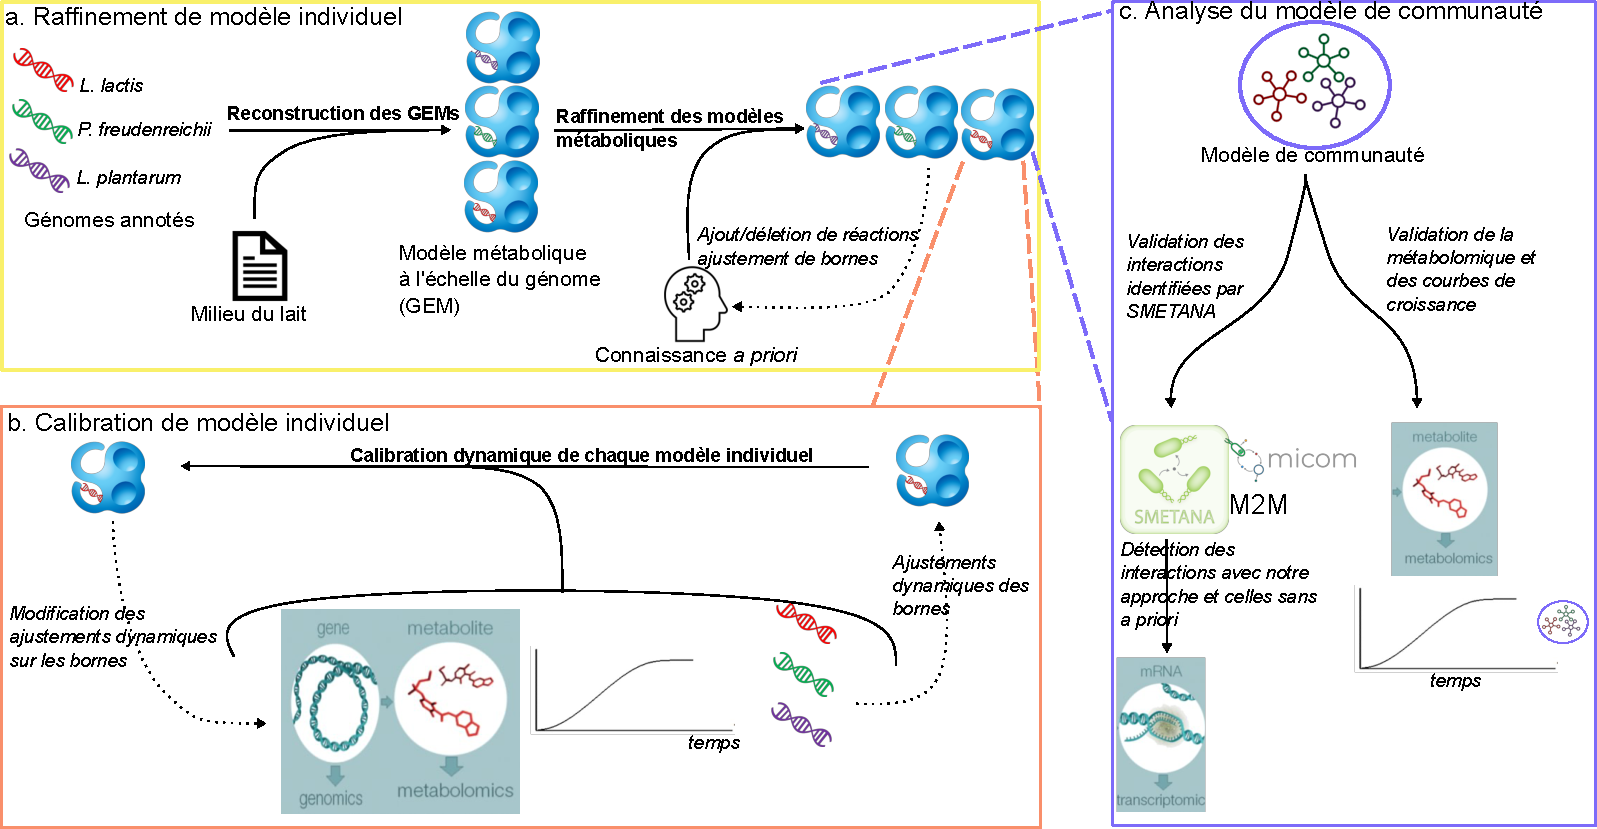
\includegraphics[width=\textwidth]{img/tango/global.pdf}
    \caption{Récapitulatif des étapes de raffinement et de calibration des modèles métaboliques, des simulations ainsi que des données utilisées}
    \label{fig:my_label}
\end{figure}

\subsection{A l'échelle de chaque souche}


\subsubsection*{Raffinement des modèles FBA individuels}
Les réseaux métaboliques à l'échelle du génome ont été reconstruits pour chaque souche individuelle depuis leurs séquences génomiques annotées respectives. Après une première étape automatique de reconstruction faite avec CarveMe, nous avons tout d'abord ajusté les flux des métabolites présents dans les réseaux métaboliques en cohérence avec la composition du lait. Les bornes inférieures de réactions d'échanges de composés qui n'apparaissent pas dans la composition du lait, sont ainsi mises à 0. La liste est constituée des réactions d'échange du glucose ($EX\_glc\_\_D\_e$) et du coenzyme A ($EX\_coa\_e$) pour \lactis et \plantarum, de l'amidon  ($EX\_starch1200\_e$) pour \lactis et \freud, du dihydroxyacetone  ($EX\_dha\_e$) pour \plantarum et \freud et du galactose ( $EX\_gal\_\_e$) pour \plantarum. \\


Nous avons ensuite réalisé un raffinement manuel du métabolisme carboné central basé sur la littérature et la connaissance biologique dans le but de prendre en compte les spécificités de chaque souche bactérienne. Le métabolisme carboné central produit du NADH and NADPH et ses formes réduites correspondantes, de l'ATP, et les précurseurs nécessaires pour la biosynthèse des molécules essentielles pour la croissance ainsi que pour l'activité métabolique des cellules bactériennes, e.g. acides aminés, purine, pyrimidine, glycerol-3-phosphate, acides gras, N-acetyl-glucosamine, vitamines. Parmi les voies métaboliques du métabolisme carboné central, la glycolyse et la voie des pentose phosphate sont communes aux trois espèces et presque identiques. Les sources de carbone telles que le lactose, l'acide citrique et l'acide lactique, sont converties en pyruvate, qui sera utilisé dans des voies spécifiques représentées dans les Figure \ref{figure:metabolic_map_freud},\ref{figure:metabolic_map_lactis},\ref{figure:metabolic_map_plantarum}. Dans la suite du chapitre, les caractéristiques métaboliques de chaque souche seront étudiées afin de justifier les raffinement faits, en se focalisant sur les voies métaboliques secondaires permettant la production de composés organoleptiques.


\paragraph*{Bactéries lactiques}
Les bactéries lactiques \lactis et \plantarum utilisent le lactose et le citrate, les deux principales sources de carbone du lait \citep{Widyastuti2014}. Le lactose est dégradé par l'enzyme beta-galactosidase en galactose et glucose, et ce dernier alimentent la glycolyse. Concernant le galactose et l'acide citrique, leur métabolisme dépend de la souche étudiée \citep{Palles1998}. D'un coté, le lactose est converti en glucose-6-phosphate \textit{via} la voie métabolique de Leloir avant d'entrer dans la glycolyse, et de l'autre l'acide citrique est converti en pyruvate par l'enzyme citrate lyase \citep{alma991000892589705596}. Du point de vue du métabolisme secondaire, le butanediol et le diacétyle sont responsables de la saveur beurrée du fromage, et sont produits par les deux modèles à partir du pyruvate grâce à la voie de l'acétolactate. L'ensemble des voies métaboliques décrites ci-dessus est récapitulé dans les Figures \ref{figure:metabolic_map_lactis} et \ref{figure:metabolic_map_plantarum}. \\



\subparagraph*{\lactis}
Pour permettre la production de certains composés d'intérêt, comme le butanediol, le GEM a été manuellement curé (Fig.~ \ref{figure:metabolic_map_lactis}). En reprenant la méthode de raffinement de modèle décrite plus haut, le flux de l'acétoine-dehydrogenase a été bloqué (ACTD2) permettant la production du butanediol. Les bornes de l'acétolactate decarboxylase (ACLDC) et de l'acétolactate synthase (ACLS) ont été modifiées de façon à permettre l'activation de la voie de l'acetolactate, comme retrouvé dans la littérature \citep*{Carroll1999,Swindell1996,Makhlouf2006}. Enfin, la consommation de lactose a été régulée en modifiant les bornes de la réaction LACZ ce qui a permis un flux de production de lactate pour \lactis (Fig.~ \ref{figure:metabolic_map_lactis}.

Pour valider ce modèle, nous avons considéré un exemple d'activation de voie métabolique durant la production du fromage, validable au regard de la littérature et des données de métatranscriptomiques. Il est montré que \lactis consomme le lactose à la fois par la voie du tagatose, codée dans l'opéron plasmidique \textit{lacABCD}, ou par la voie de Leloir, codée dans l'opéron du chromosome \textit{galKTE}. D'un point de vue des données metatranscriptomiques, \lactis exprime les gènes associés à la voie du tagatose au début de la production de fromage quand la concentration de lactose est grande, et ceux de la voie de Leloir durant l'affinage quand la concentration de lactose est faible. Cela suggère fortement que la concentration de lactose détermine quelle voie métabolique est employée, et prédit qu'une grande quantité de lactose dans le milieu nutritionnel devrait produire un flux important à travers la voie du tagatose. Le modèle FBA de \lactis est en accord avec les données métatranscriptomiques. Nous avons observé un flux important de dégradation du lactose à travers la voie du tagatose (Fig. \ref{dfba_metabolite_lactis}~a).

\begin{figure}[H]
    \centering
    % \hspace{-3.5cm}
    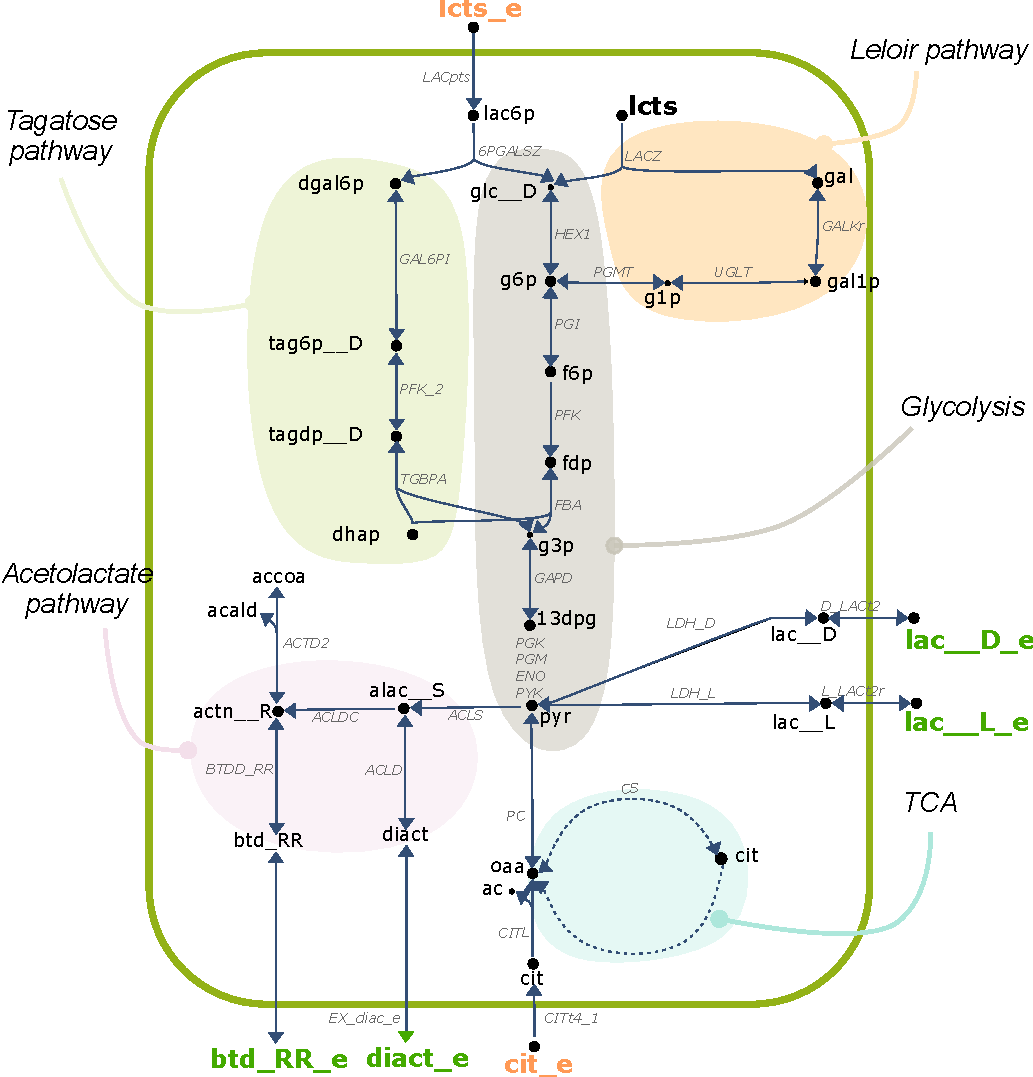
\includegraphics[width=1\textwidth]{img/tango/carte_lactis.pdf}
    \caption{\textbf{Cartes des voies métaboliques du métabolisme carboné central d'intérêt de \textit{L. lactis}}. La voie métabolique de la glycolyse est représentée en gris, celle de Leloir en saumon, acétolactate en rose, le cycle du TCA en bleu clair, et le tagatose en vert. Les métabolites en orange et vert correspondent aux entrées et sorties du modèle métabolique. La liste des métabolites et des réactions est répertoriée à la fin du chapitre à la section \ref{abbreviation-metabo} }
    \label{figure:metabolic_map_lactis}
\end{figure}

\subparagraph*{\plantarum}
L'exemple pris pour \plantarum concerne la dégradation du glucose et du galactose dans le cas des fermentations homolactique et hétérolactique (voir figure \ref{figure:metabolic_map_plantarum}. Dans les deux configurations, le pyruvate est produit à partir de la dégradation du glucose et du galactose. Durant la fermentation homolactique, le pyruvate est associé au relargage de l'acide lactique dans le milieu extracellulaire. Concernant la fermentation hétérolactique, on observe en plus une production d'éthanol et d'acétate. Nous savons que \plantarum est une bactérie hétérolactique pouvant produire de l'acétate grâce à l'enzyme transketolase (numéro EC 4.1.2.9) décrit dans \citep{Abedi2020} à travers la voie métabolique de l'acétate kinase. Pour permettre cette production dans notre modèle, nous avons bloqué la pyruvate formate lyase (PFL) \citep{Quatravaux2006}. Concernant le butanediol, la même curation que pour \lactis a été effectuée. Enfin, pour reproduire la dégradation du galactose et du glucose par la voie de Leloir et de la dégradation du lactose grâce à la $\beta$-galactosidase \textit{LACZ}, la réaction \textit{LCTSt3ipp} a été bloquée et la réaction UTP-glucose-1-phosphate uridylytransferase (\textit{GALUi}) a été rendue réversible pour compléter la voie de dégradation du galactose (Fig. \ref{dfba_metabolite_plant}~a).


\begin{figure}[H]
    \centering
    % \hspace{-3.5cm}
    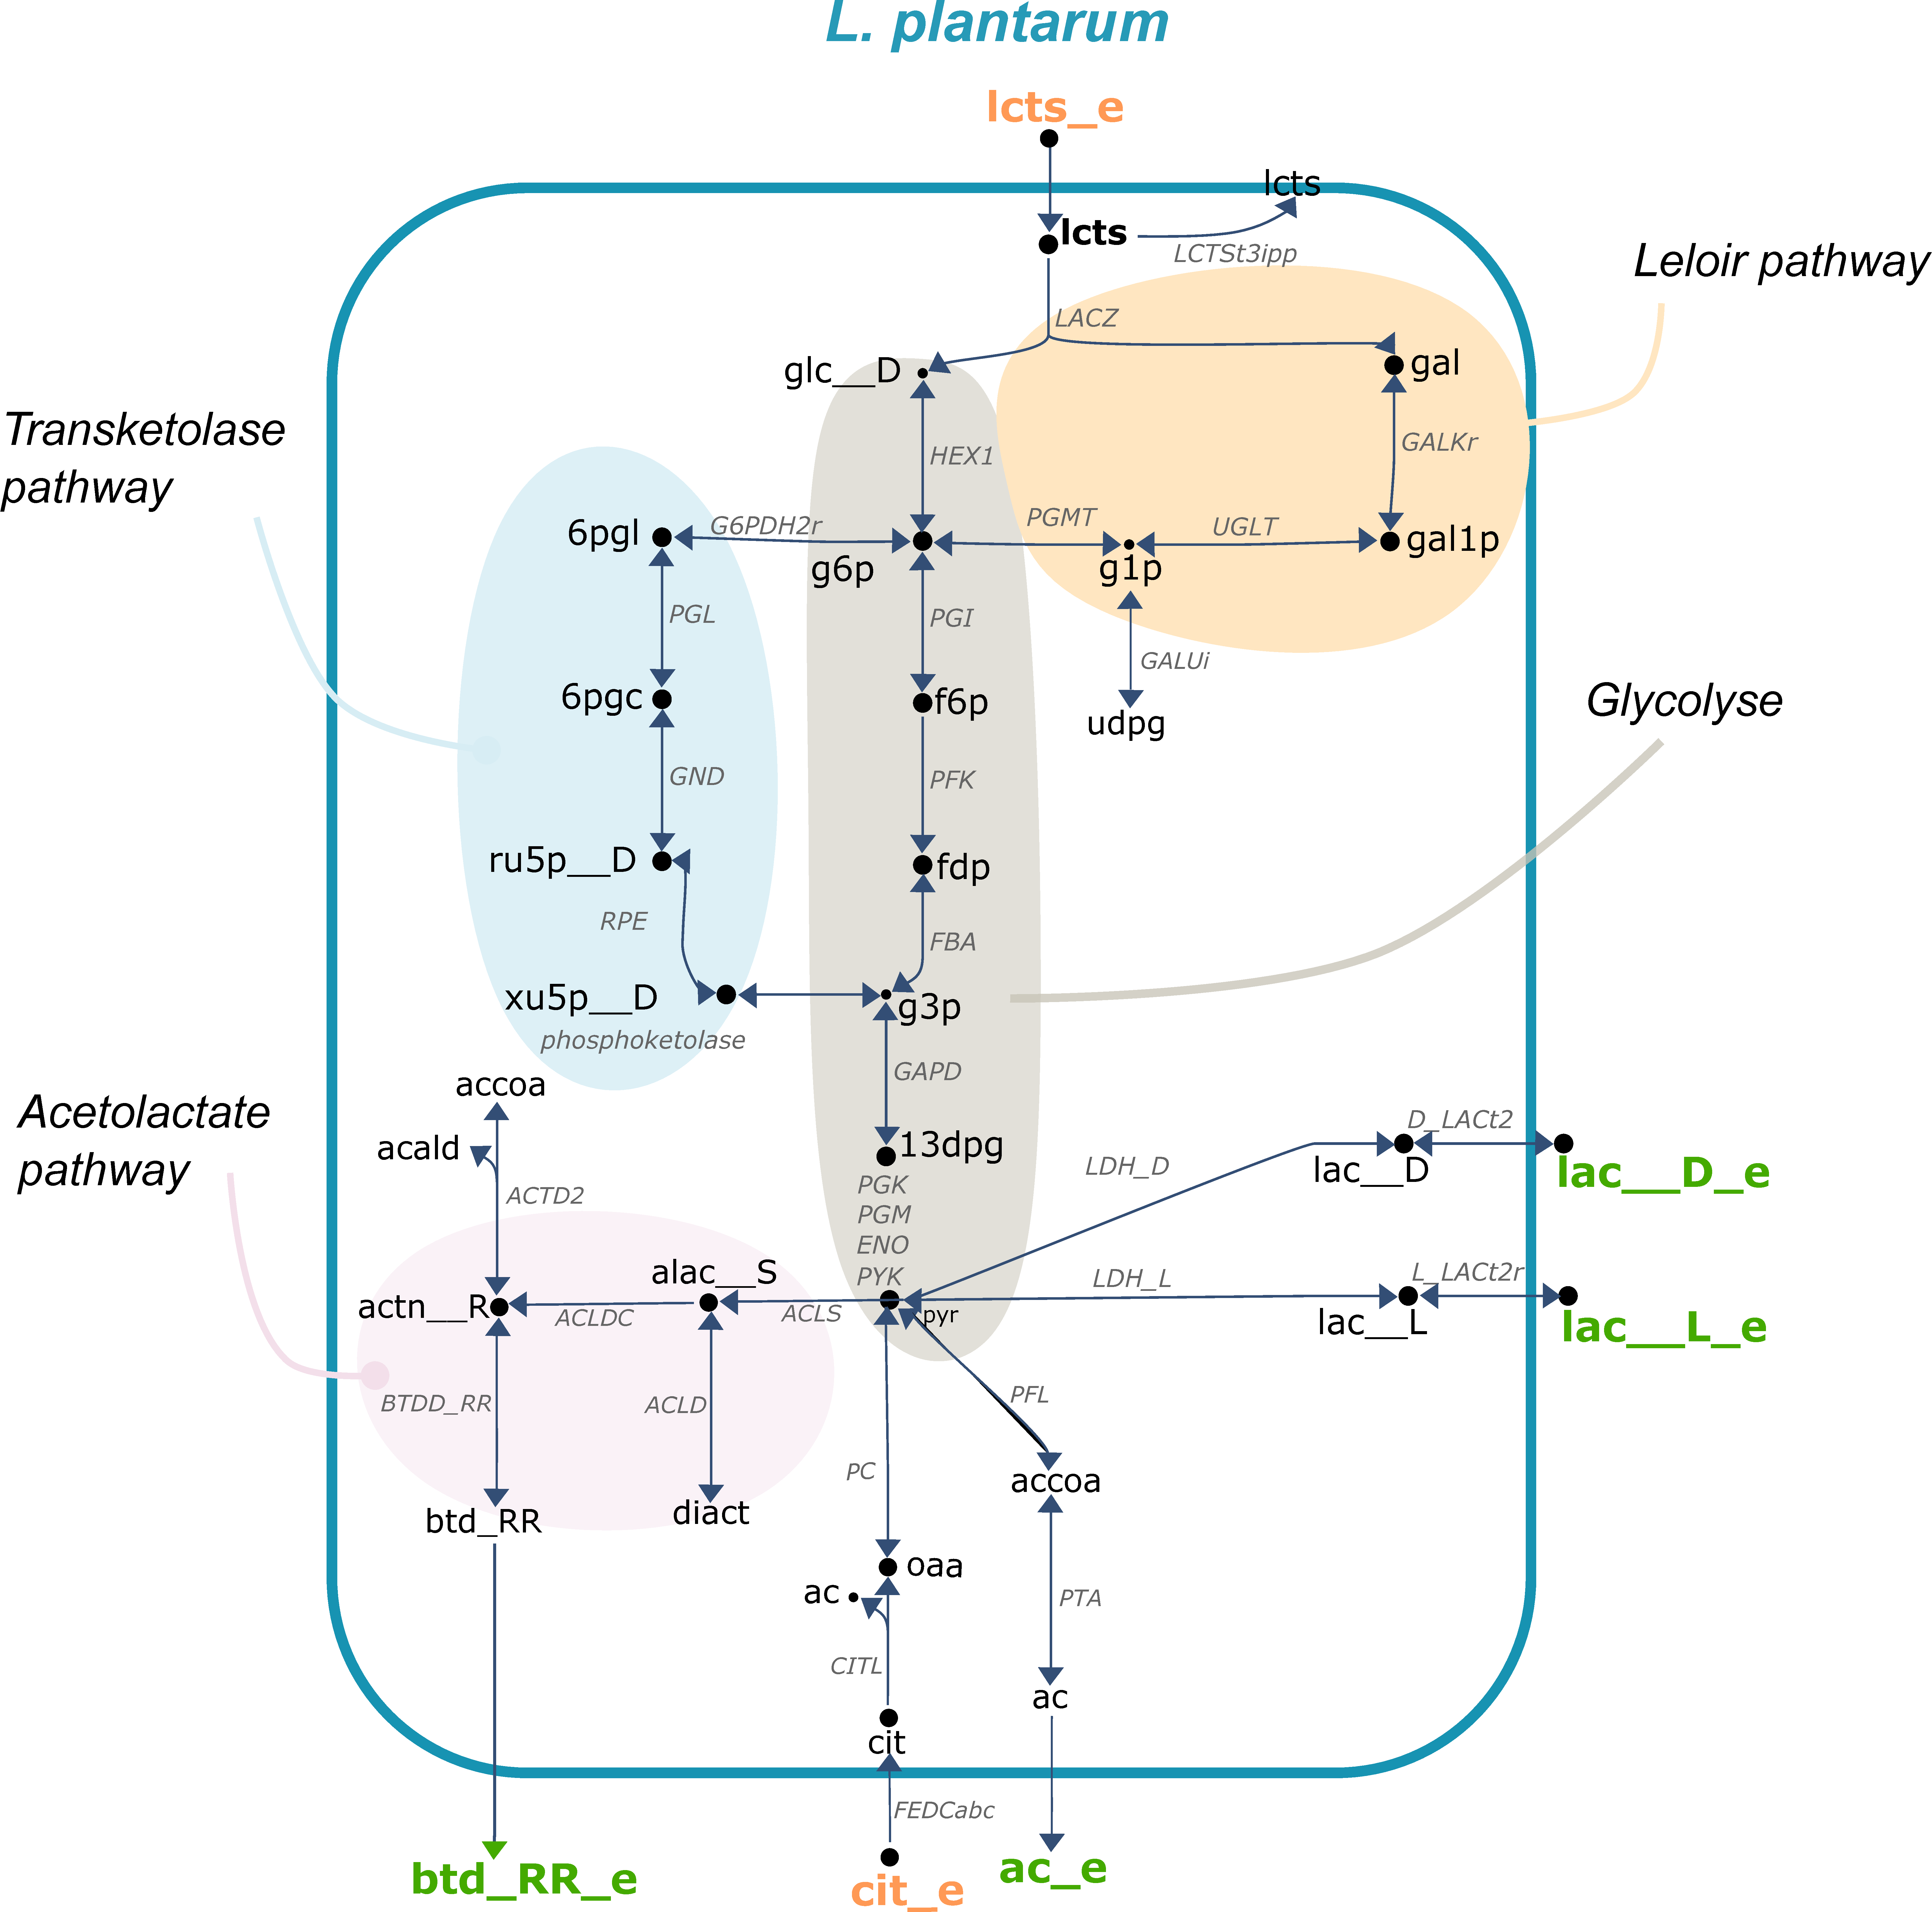
\includegraphics[width=1\textwidth]{img/tango/carte_plantarum.pdf}
    \caption{\textbf{Cartes des voies métaboliques  du métabolisme carboné central d'intérêt de \textit{L. plantarum}}. La voie métabolique de la glycolyse est représentée en gris, celle de Leloir en saumon, acétolactate en rose, et la transketolase en bleue. Les métabolites en orange et vert correspondent aux entrées et sorties du modèle métabolique. La liste des métabolites et des réactions est répertoriée à la fin du chapitre à la  section \ref{abbreviation-reac}}
    \label{figure:metabolic_map_plantarum}
\end{figure}

\paragraph*{\freud}

La souche CIRM-BIA122 de \freud consomme à la fois l'acide lactique, sa principale source de carbone \citep*{Thierry2011,Dank2021} et/ou le lactose \citep{Loux2015}. L'acide lactique et le lactose sont catabolisés par les voies de la glycolyse et des pentose-phosphate, menant à la production de pyruvate. Une part du pyruvate alimente le cycle des acides  tricarboxylique (TCA) et la voie de Wood-Werkman  (Fig.~\ref{figure:metabolic_map_freud}) dans laquelle l'acide propionique peut être produit. Cette voie métabolique est spécifique au genre \textit{Propionibacterium} et est assurée en redirigeant le succinate à partir du TCA. Les productions d'acide acétique et du CO$_2$ \citep{Turgay2020} à partir du pyruvate sont permises grâce à l'activité de la pyruvate oxidase et de la pyruvate dehydrogenase respectivement. Pour assurer la proportion correcte de propionate/acétate, le GEM de \freud a requis de plus amples curations. En effet, les bornes des réactions \textit{PPAKr}, \textit{PTAr}, \textit{2131pyrpp} ont été modifiées pour orienter le métabolisme vers la voie de  Wood-Werkman, et la réaction \textit{POX2} a été bloquée pour réguler le flux d'acétate.

Un moyen de valider nos modifications est de calculer le ratio de concentration de propionate sur l'acétate afin de vérifier si ce dernier coïncide avec les observations biologiques. Nous avons obtenu la valeur de 2.19, ce qui est confirmé par ratio de 2 trouvé dans les travaux de  \citep*{Crow1986,Dank2021,Cao2021, Turgay2020}. \\ 

L'ensemble des modifications portées à chaque modèle métabolique est résumé dans la table \ref{table:manual-refinement}.

\begin{figure}[H]
    \centering
    % \hspace{-3.5cm}
    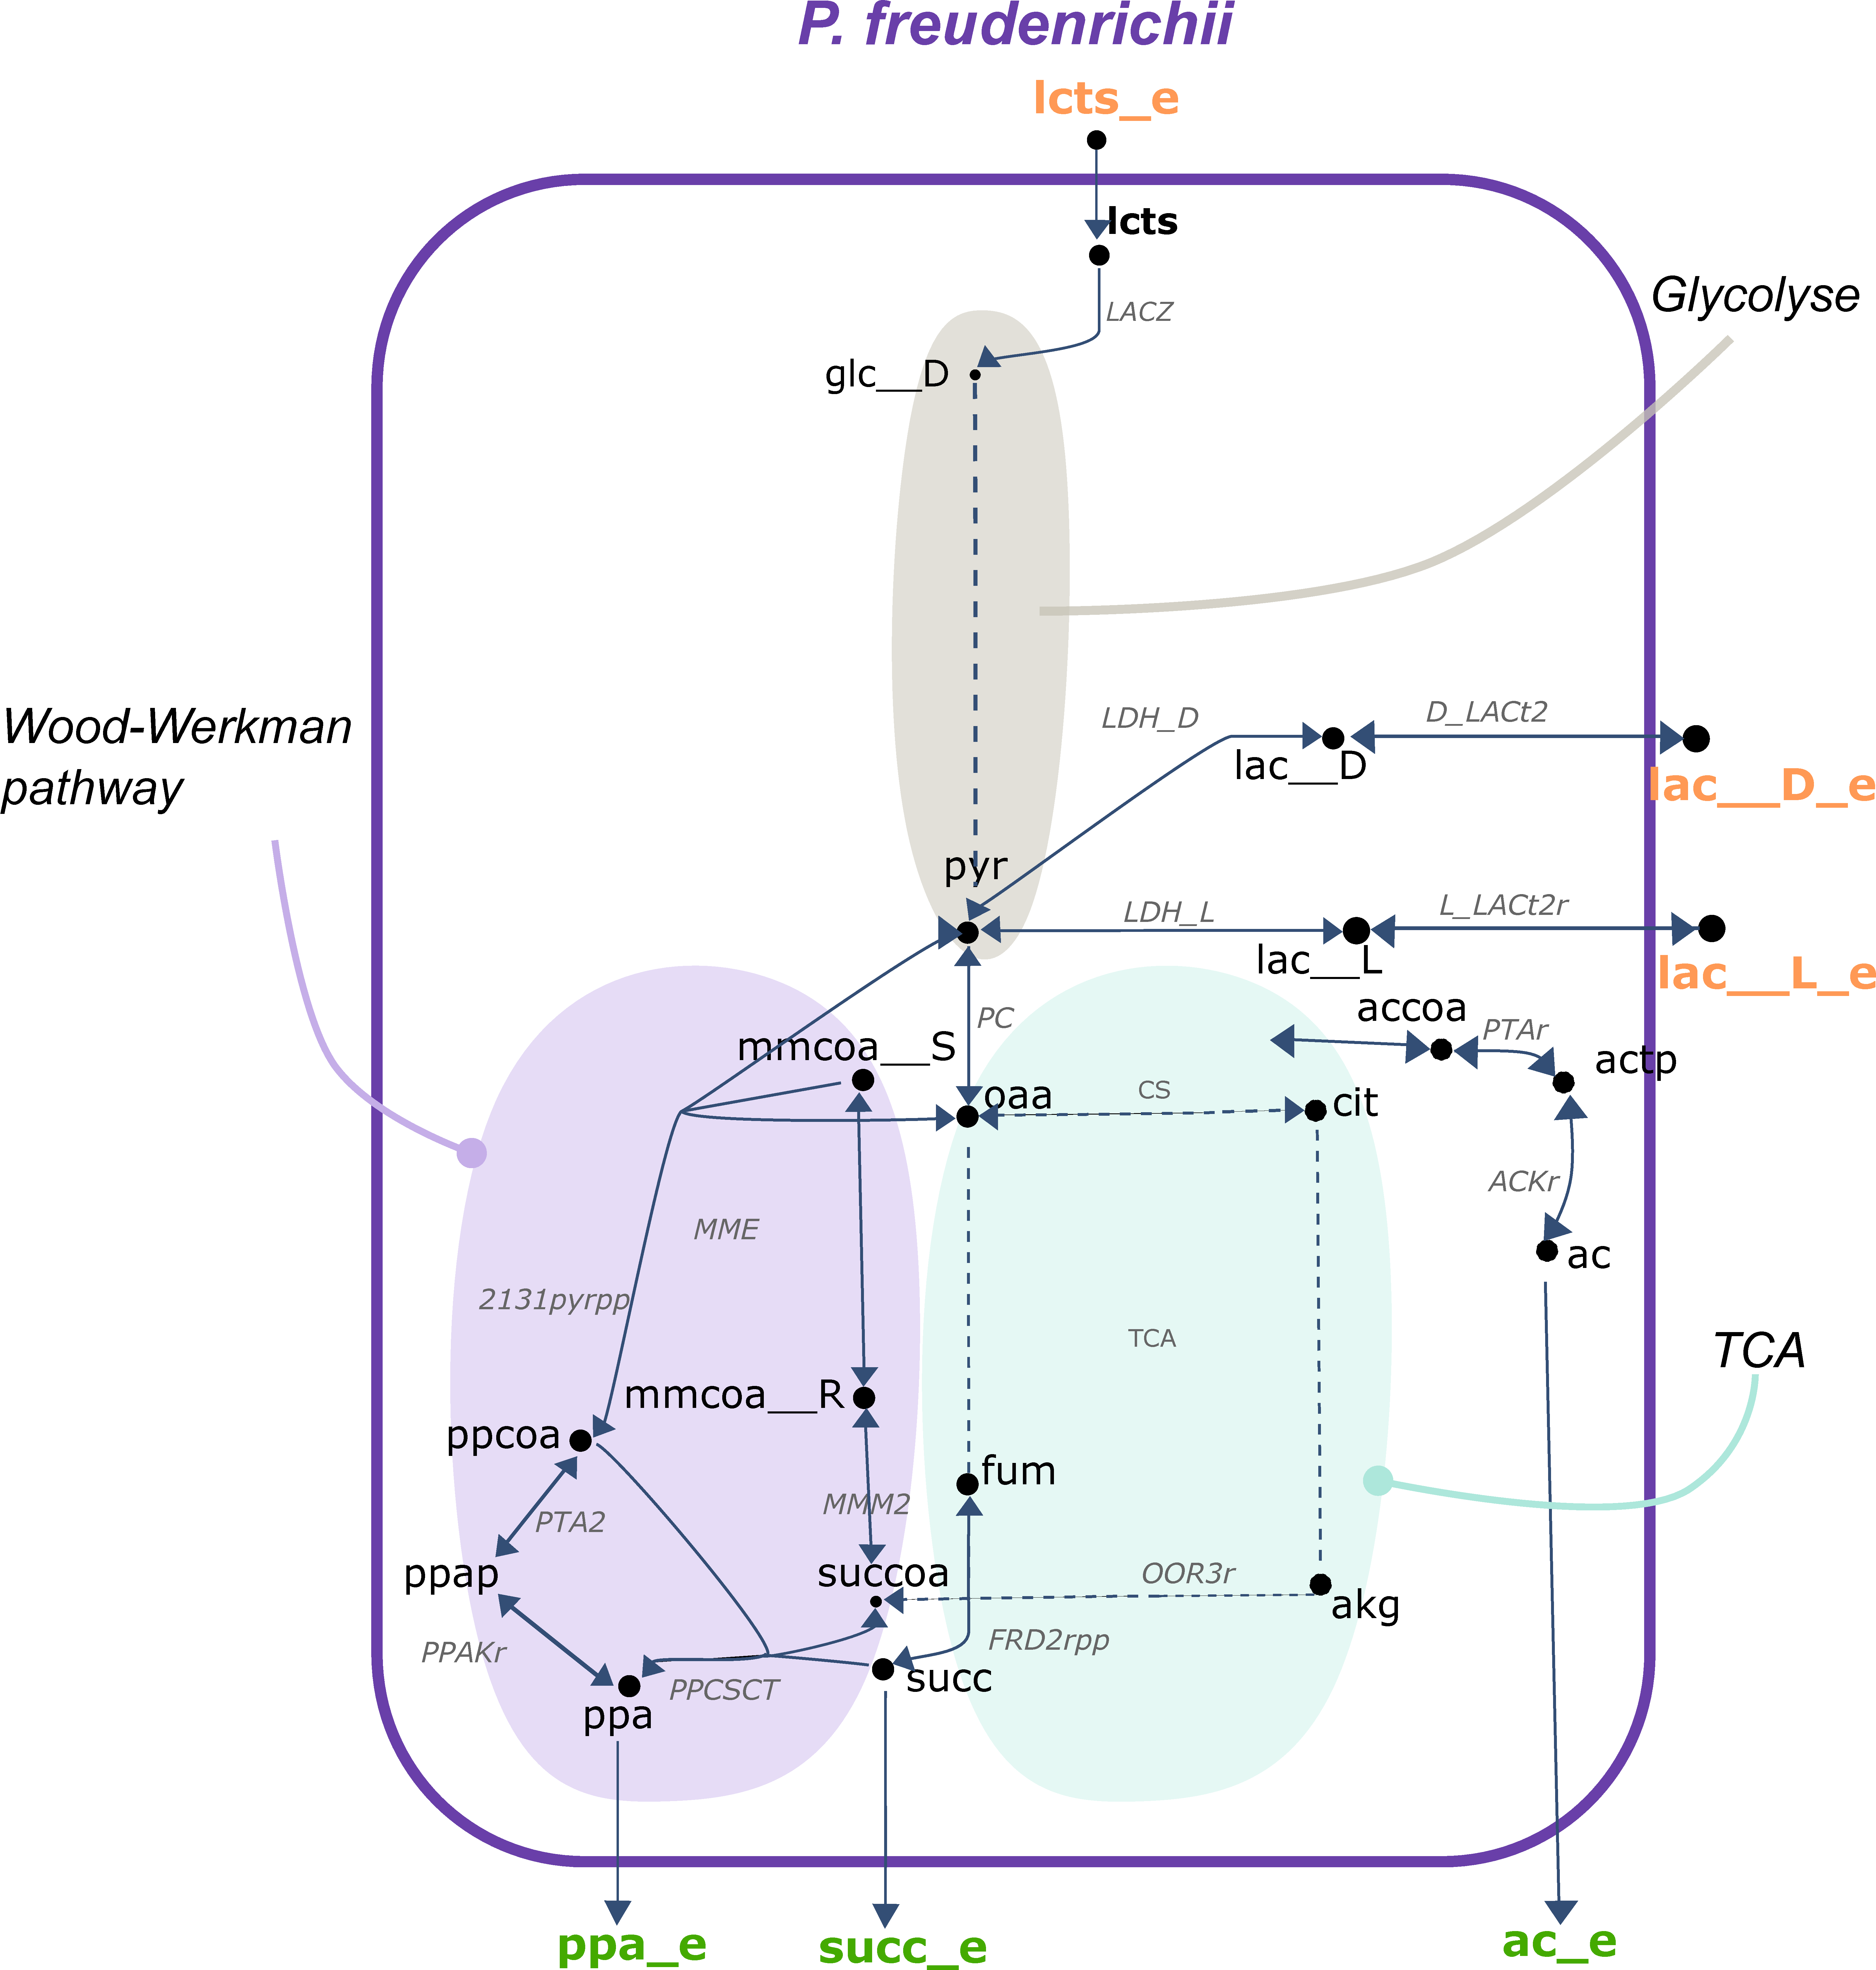
\includegraphics[width=1\textwidth]{img/tango/carte_freud.pdf}
    \caption{\textbf{Cartes des voies métaboliques du métabolisme carboné central  d'intérêt de \textit{P. freudenreichii}}. La voie métabolique de la glycolyse est représentée en gris, le cycle du TCA en bleu clair, et la voie de Wood-Werkman en violet. Les métabolites en orange et vert correspondent aux entrées et sorties des modèles métaboliques. La liste des métabolites et des réactions est répertoriée à la fin du chapitre à la section \ref{abbreviation-reac}}
    \label{figure:metabolic_map_freud}
\end{figure}



Nous avons par la suite vérifié la qualité de chaque réseau métabolique: une faible fraction de réactions universellement bloquées (< 3\%), et une faible fraction de réactions sans association de gène-proteine-réactions (GPR) (< 30\%) \citep{Lieven.2020}. Puis, nous les avons analysés par la méthode d'équilibre des flux (FBA) \citep{Palsson1994,Orth2010} assurant ainsi la production des molécules de la biomasse à partir de l'environnement nutritionnel du lait. Nous avons obtenu des taux de croissances allant de 0.187 $\text{mmol.gDW}^{-1}\text{.hr}^{-1}$ pour \freud à 2.17 $\text{mmol.gDW}^{-1}\text{.hr}^{-1}$ pour \lactis. Comme les conditions dans le fromage correspondent à des conditions de microaérobiose \citep{Miyoshi2003}, une attention particulière a été donnée au rôle de l'oxygène sur le métabolisme des trois bactéries en modifiant la borne supérieure de la réaction d'importation dans le compartiment cytosolique. Les caractéristiques générales des trois modèles sont décrites dans la Table \ref{tab:table1}. Nous observons que \lactis a un plus petit nombre de réactions que les deux autres souches, une différence qualitative qui est aussi observée pour les autres souches de la même espèce dans d'autres bases de données \citep{Noronha.2018}.\\


\begin{center}
    \begin{table}[h!]
    \begin{tabular}{|l|c|c|c|}
    \hline
                                                                                & \textit{P. freudenreichii} & \textit{L. plantarum} & \textit{L. lactis} \\ \hline
    Nombre de gènes                                                                                     & 1473                       & 1433                  & 1272               \\ \hline
    Nombre de métabolites                                                                               & 1284                       & 1045                  & 939               \\ \hline
    Nombre de réactions                                                                                 & 1790                       & 1523                  & 1337               \\ \hline
    \begin{tabular}[c]{@{}l@{}}Pourcentage de réactions\\  associées a au moins un gène \end{tabular} & 76.6                       & 79.0                    & 82.1               \\ \hline
    \begin{tabular}[c]{@{}l@{}}Taux de croissance en $\text{mmol.gDW}^{-1}\text{.hr}^{-1}$\end{tabular}                           & 0.187                       & 0.645                  & 2.172                \\ \hline
    \end{tabular}
    \caption{Caractéristiques générales des 3 modèles métaboliques}
    \label{tab:table1}
    \end{table}
\end{center}




\begin{table}[h!]
\begin{adjustbox}{width=1\textwidth}
\begin{tabular}{|c|c|c|c|c|}
\hline
GEM & Reaction & Bornes & Valeur & Justification \\
 \hline
 \TableBac{\lactis}{8} & \TableReac{ACTD2}{borne inférieure}{0}{borne supérieure}{0}{Permet l'activation de la voie métabolique de l'acetolactate}\\
 \cline{2-5}
 & \TableReac{ACLDC}{borne inférieure}{0}{borne supérieure}{2}{Permet l'activation de la voie métabolique de l'acetolactate}\\
 \cline{2-5}
 & \TableReac{ACLS}{borne inférieure}{2}{borne supérieure}{1000}{Permet l'activation de la voie métabolique de l'acetolactate}\\
 \cline{2-5}
 & \TableReac{LACZ}{borne inférieure}{0.0006}{borne supérieure}{2}{Oblige la consommation de lactose}\\ 
 \hline
 \TableBac{\plantarum}{10} & \TableReac{PFL}{borne inférieure}{0}{borne supérieure}{0}{Permet la production des deux isomères de lactate à partir du lactose} \\
 \cline{2-5}
 & \TableReac{LCTSt3ipp}{borne inférieure}{0}{borne supérieure}{0}{Redirige le flux de lactose dans la voie métabolique de la Glycolyse}\\
\cline{2-5}
 & \TableReac{ACTD2}{borne inférieure}{0}{borne supérieure}{0}{Permet l'activation de la voie métabolique de l'acetolactate}\\
 \cline{2-5}
 & \TableReac{GALUi}{borne inférieure}{-30}{borne supérieure}{10}{Permet la production des deux isomères de lactate à partir du lactose}\\
 \cline{2-5}
 & \TableReac{ACLS}{borne inférieure}{2}{borne supérieure}{1000}{Permet l'activation de la voie métabolique de l'acetolactate}\\
 \hline
 \TableBac{\freud}{14} & \TableReac{6PGALSZ}{borne inférieure}{0}{borne supérieure}{0}{Réaction appartenant à la voie du tagatose, non présente chez \freud} \\
 \cline{2-5}
 & \TableReac{XYLI2}{borne inférieure}{0}{borne supérieure}{0}{\begin{minipage}[t]{0.6\linewidth}A partir du glucose, le fructose était produit à la place du glucose-6-phosphate et la Glycolyse n'était pas activée.\end{minipage}}\\
\cline{2-5}
 & \TableReac{POX2}{borne inférieure}{0}{borne supérieure}{0}{Régule le flux d'acétate}\\
 \cline{2-5}
 & \TableReac{PPAKr}{borne inférieure}{0}{borne supérieure}{0}{Inhibe la surproduction de l'acétate}\\
 \cline{2-5}
 & \TableReac{LACZ}{borne inférieure}{0}{borne supérieure}{5}{Autorise la consommation de lactose}\\
  \cline{2-5}
 & \TableReac{PTAr}{borne inférieure}{-1000}{borne supérieure}{8}{Permet d'obtenir le bon ratio de production propionate/acetate}\\
  \cline{2-5}
 & \TableReac{2131pyrpp}{borne inférieure}{8}{borne supérieure}{1000}{Permet d'obtenir le bon ratio de production propionate/acetate}\\
\hline
\end{tabular}
\end{adjustbox}
\caption{\textbf{Raffinement manuel des GEMs avec les justifications correspondantes} \label{table:manual-refinement}}
\end{table}


Le raffinement des trois modèles FBA a permis la prédiction de production et de consommation de plusieurs composés d'arômes tels que les acides lactique, acétique et propionique, le diacétyl et le butanediol \citep{Smid2014, Cao2021} (Fig.~\ref{figure:metabolic_map_freud},\ref{figure:metabolic_map_lactis},\ref{figure:metabolic_map_plantarum}). De plus, les spécificités métaboliques de chaque souche en fonction de leur métabolisme primaire ont été reproduites fidèlement: la voie de Wood-Werkman pour \freud, la voie du tagatose pour \lactis et la voie de la transketolase pour \plantarum.  \\


La méthode itérative a permis de répondre à la première exigence que le modèle numérique doit satisfaire: "vérifier que les voies métaboliques d'intérêts  permettant la production des composés d'arômes soient présentes et activées". Nous avons reproduit de manière qualitative, la production et la consommation de métabolites connues de la littérature. Nous avons également prédit de nouveaux comportements métaboliques, comme la dégradation du citrate chez \plantarum par les enzymes de la famille CITL. Afin d'obtenir des prédictions numériquement proches des courbes de croissance et des concentrations de métabolites, nous avons ensuite calibré chaque modèle individuel.

\subsubsection*{Calibration dynamique}
Afin d'obtenir des modèles individuels suffisamment bien curés, nous avons utilisé les données cinétiques à disposition pour affiner chaque modèle (voir \ref{données-calibration}). Cette étape de calibration consiste à minimiser l'écart entre les données expérimentales et la simulation de façon dynamique en estimant des paramètres (voir \ref{table:manual-refinement}). Pour ce faire, le modèle numérique devait permettre: d'intégrer des données hétérogènes et de modéliser la dynamique de croissance et de production/consommation de métabolites pour chaque souche.

L'objectif à atteindre est de retrouver numériquement les observations biologiques que sont: la croissance bactérienne,  l'évolution du pH pour \lactis et \plantarum ainsi que les concentrations des métabolites pour \freud. \\

Pour estimer les paramètres, nous avons résolu le problème de minimisation décrit dans les équations \ref{eq:optim_LAB} pour les bactéries lactiques et \ref{eq:optim_freud} pour \freud. Brièvement, nous cherchons à minimiser l'écart aux données de croissance pour les 3 espèces, l'écart aux données de pH pour les deux bactéries lactiques et l'écart aux données de dosage de métabolites pour \freud. Avec ce type de méthode, le sur-apprentissage, est une problématique à prendre en compte. Afin de l'éviter, nous avons optimisé un petit nombre de paramètres pour chaque espèce : seulement deux paramètres ont été utilisés pour calibrer la croissance de \lactis et la régulation du pH, trois pour \plantarum régulant le pH ainsi que sa croissance, et enfin, un paramètre pour \freud, ajustant sa croissance.\\

Ce principe de calibration des modèles se base également sur un processus itératif induit par les allers-retours entre les données simulées et les paramètres inférés. En effet, la solution informatique d'optimiser des paramètres pour ajuster les modèles n'est pas suffisante. Nous avons dû établir des contraintes de modélisation dynamique en se basant sur la connaissance biologique de l'espèce ainsi que sur les résultats des simulations. Expérimentalement, nous avons observé que le métabolisme des bactéries lactiques est toujours actif pendant la phase stationnaire au regard de la courbe de pH, indiquant que les bactéries continuent d'acidifier. Elles peuvent ainsi continuer de produire du lactate et de l'acétate à partir du lactose puisque ce dernier n'est pas considéré comme limitant dans les conditions expérimentales. La première contrainte dynamique a consisté à réguler le flux de production des acides lactique et acétique par le flux de consommation du lactose, source de carbone principale. 

\paragraph*{\lactis et \plantarum}
Pour moduler le flux de production des acides lactique, les bornes supérieures des réactions d'échange du lactate EX\_lac\_\_L\_e et EX\_lac\_\_D\_e, sont modulées comme suit:

\begin{equation}
min(\frac{m_{lcts_e}}{\Delta t*\sum_{i \in \mathcal{M}(lcts_e)} b_i},\mu_{max,lcts}*10^{(-k_{lac}*\phi_{undiss})}+\mu_{min,lcts})*4
\label{eq:lactate_lactis}
\end{equation}

Toutes les constantes sont décrites dans la sous section \ref{dynamic analyse}. Pour rappel, $m_{lcts_e}$ est la concentration du lactose, $\mathcal{M}(lcts_e)$ le sous ensemble des bactéries métabolisant le lactose, $\mu_{max,lcts}$ et $\mu_{min,lcts}$ valeurs maximales et minimales de consommation du lactose, $k_{lac}$ une décroissance exponentielle et $\phi_{undiss}$ la fonction qui calcule la concentration de la forme non dissociée de l'acide lactique à partir du lactate.

Comme la production de lactate est reliée à la disponibilité du lactose, nous avons modulé dynamiquement l'export de lactate en fonction de la quantité de lactose à importer, avec un coefficient st\oe{}chiométrique de 4 (voir eq.~\eqref{eq:lactose_lab}). Ce coefficient permet de mieux ajuster la courbe de production de lactate aux données expérimentales.\\

Étant donné que l'acétate n'est pas relié dans notre modèle au calcul du pH, mais est produit à partir du lactose par l'intermédiaire du pyruvate, nous avons appliqué une simple régulation de la production de l'acétate par la quantité de lactose disponible. Soit EX\_ac\_e, la réaction d'échange de l'acétate, sa borne supérieure sera modulée dynamiquement par:

\begin{equation*}
max(-\frac{m_{lcts_e}}{\Delta t*\sum_{i \in \mathcal{M}(lcts_e)} b_i},v^{exp}_{i,ac_e})
\end{equation*}

La production d'acétate est régulée par la disponibilité de lactose quand celui ci est épuisé, représenté par $-\frac{m_{lcts_e}}{\Delta t*\sum_{i \in \mathcal{M}(lcts_e)} b_i}$ , autrement sa production sera limitée par sa limite d'export physiologique intrinsèque $v^{exp}_{i,ac_e}=0.5$ pour \lactis et $v^{exp}_{i,ac_e}=1.0$ pour \plantarum. \\

Lorsque les concentrations extra-cellulaires de lactose sont suffisamment importantes, le flux de consommation du lactose par les bactéries lactiques est également régulé par l'acidité libérée par ces bactéries: $-\mu_{max,lcts}*10^{(-k_{lac}*\phi_{undiss})}-\mu_{min,lcts}$. En effet, le métabolisme des bactéries lactiques continue même lorsqu'elles sont à l'état stationnaire. En revanche, lorsque la concentration de lactose devient insuffisante, un partage uniforme entre les bactéries consommatrices, composées des deux bactéries lactiques et de la bactérie propionique est mis en place: $-\frac{m_{lcts_e}}{\Delta t*\sum_{i \in \mathcal{M}(lcts_e)} b_i}$. L'approche modélisant ce processus est inspirée des travaux de \citep{Ozcan.2020} dans lesquelles l'acidité libérée par les bactéries lactiques est représentée par le forme non dissociée de l'acide lactique.\\

Soit EX\_lcts\_e, la réaction d'échange du lactose. Sa borne inférieure des bactéries lactiques sera modulée dynamiquement par:

\begin{equation}
max(-\frac{m_{lcts_e}}{\Delta t*\sum_{i \in \mathcal{M}(lcts_e)} b_i},-\mu_{max,lcts}*10^{(-k_{lac}*\phi_{undiss})}-\mu_{min,lcts})
\label{eq:lactose_lab}
\end{equation}

Concernant la régulation par le pH, la quantité d'acide lactique non dissocié est calculé à partir de la concentration de lactate au moyen de la fonction $\phi_{undiss}$ (voir équation \ref{eq:undissociated-lactate} pour l'expression de cette fonction); puis, avec une croissance exponentielle à partir de la valeur $-\mu^{lact}_{max,lcts}-\mu^{lact}_{min,lcts}$ (respectivement $-\mu^{plant}_{max,lcts}-\mu^{plant}_{min,lcts}$ pour \plantarum) à la valeur $-\mu^{lact}_{min,lcts}$ ($-\mu^{plant}_{min,lcts}$) quand la concentration d'acide lactique non dissocié augmente, avec un taux exponentiel $k_{lac}$. Les valeurs de $\mu^{lact}_{max,lcts}$ (resp. $\mu^{plant}_{max,lcts}$), $\mu^{lact}_{min,lcts}$ (resp.$\mu^{plant}_{min,lcts}$) et $k_{lac}$ sont inférées à partir des expériences de co-cultures. \\


Pour \freud, lorsque le lactose est épuisé numériquement, nous avons appliqué le même partage uniforme des ressources que pour les bactéries lactiques : $-\frac{m_{lcts_e}}{\Delta t*\sum_{i \in \mathcal{M}(lcts_e)} b_i}$. Sinon, comme il n'est pas impacté par sa propre acidification, un flux constant $F_{lcts}$ estimé des données de métabolomiques en culture pure est appliqué lorsque la quantité de lactose est suffisamment abondante. Ce flux constant est estimé de la façon suivante:
\begin{equation}
\label{sec:estimate-bounds-freud}
 {\mu}_{i,j} = \alpha \frac{ m_j(T)-m_j(0)}{\int_0^T b_i(t) dt}
\end{equation}
 
où ${\mu}_{i,j}$ correspond à la valeur de flux,  $m_j$ la concentration du métabolite, $T$ valeur finale, $0$ valeur initiale, $b_i(t)$ la densité bactérienne, et $\alpha$, un coefficient prenant en compte les erreurs d'approximation.


%Concernant \freud, lorsque le concentration de lactose est épuisé nous avons appliqué le même partage uniforme que pour les bactéries lactiques: $-\frac{m_{lcts_e}}{\Delta t*\sum_{i \in \mathcal{M}(lcts_e)} b_i}$. 


La borne supérieure du lactose pour chaque bactérie reste inchangée. \\

%Nous avons utilisé jusqu'ici uniquement la connaissance apportée par la littérature afin de contraindre chaque modèle individuel en y associant une équation de régulation. Dans les paragraphes suivants, une communication entre les données et les modèles sera utilisée afin d'ajouter des contraintes et expliquer les données observées pour chaque souche.\\ 

Pour rappel, le lactate, l'acétate, le succinate et le propionate sont dosés pour \freud et les concentrations initiales et finales sont récupérées. Ainsi, les bornes des flux de production de ces composés sont estimées à partir des données dans le but de rapprocher la valeur de flux de production prédite par le modèle avec celle des données expérimentales. Dans ces conditions expérimentales, les nutriments ne sont pas considérés comme limitant, ainsi nous avons modéliser la phase plateau par une croissance logistique. \\

Pour \freud, la borne de consommation du lactate est modélisée comme suit:

\begin{equation}max(-\frac{m_{lac_{L,e}}}{\Delta t*\sum_{i \in \mathcal{M}(lac_L)} b_i},F_{lac}*K_{freud}* \frac{b_{freud}}{B_{p,freud}}) \label{eq:optim-K-lac}\end{equation}

Comme précédemment avec le lactose, lorsque la quantité de lactate est insuffisante, nous avons utilisé un partage uniforme des ressources $-\frac{m_{lac_{L,e}}}{\Delta t*\sum_{i \in \mathcal{M}(lac_L)} b_i}$ parmi les bactéries consommatrice du lactate $\mathcal{M}(lac_L)$. Dans le cas contraire, un flux $F_{lac}$ estimé des données de métabolomiques en culture pure (voir l'équation \ref{sec:estimate-bounds-freud}) est appliqué après une régulation par la fraction $\frac{b_{freud}}{B_{p,freud}}$, où $B_{p,freud}$ est la valeur plateau de la concentration de la biomasse en pure culture, et $b_{freud}$ et la densité de biomasse actuelle, et le facteur $K_{freud}$, qui est inféré des données de croissance en culture pure. Cette modulation modélise un ordre de grandeur différent du rendement du métabolisme en culture pure ou en co-culture.

Comme l'acétate, le propionate et le succinate ne sont pas consommés par aucun des modèles métaboliques, seule la borne supérieure (de production) est modulée. Soient les réactions d'échanges d'acétate (EX\_ac\_e), de propionate (EX\_ppa\_e) et de succinate (EX\_succ\_e), la valeur de la borne supérieure est égale à:

\[F_{i}*K_{freud}* \frac{b_{freud}}{B_{p,freud}}, \quad \text{ pour } i \in \{\text{ EX\_ac\_e, EX\_ppa\_e,EX\_succ\_e} \}\]

où le taux maximal de production est défini par $F_{i}$, pour $i \in \{\text{ EX\_ac\_e,  EX\_ppa\_e,} $
$\text{ EX\_succ\_e} \}$ estimé à partir des données de métabolomique de culture pure (voir la section \ref{sec:estimate-bounds-freud}). Le même terme de modulation que dans l'équation \ref{eq:optim-K-lac} est appliqué, modélisant un un ordre de grandeur différent du rendement du métabolisme en culture pure ou en co-culture.\\

Cette étape itérative de calibration dynamique est coûteuse en temps. En effet, pour chacune des nouvelles valeurs de paramètres, nous avons lancé une simulation dynamique de chaque souche optimisée. 

Pour les autres métabolites suivis dynamiquement, c'est à dire le butanediol, le diacétyle et le citrate, la borne inférieure est modulée selon le principe de partage équitable décrit plus haut lorsque la quantité de substrat devient insuffisante.

Soient EX\_diact\_e, EX\_btd\_RR\_e et EX\_cit\_e les réactions d'échanges correspondantes aux diacétyle, butanediol et citrate, leurs bornes inférieures sont ainsi modulées par:

\begin{align*}
&max(-\frac{m_{j}}{\Delta t*\sum_{i \in \mathcal{M}(j)} b_i},v^{int}_{i,j})\\
&\text{ pour }i=\text{\lactis si } j \in \{EX\_diact\_e,EX\_btd\_RR\_e,EX\_cit\_e,EX\_ac\_e\}\\
&\text{ pour }i=\text{\plantarum si } j \in \{EX\_btd\_RR\_e\}
\end{align*}

%Limitation dynamique de consommation (voir eq. \eqref{eq:usual-consumption-limitation}). 
Quand le substrat n'est pas limité, l'import est contraint par la limite physiologique intrinsèque modélisé par $v^{int}_{i,j} = -8$ pour $j=$\lactis et $j \in \{EX\_diact\_e,EX\_btd\_RR\_e\}$,
$v^{int}_{i,j} = -1$ pour $j=EX\_cit\_e$ et $v^{int}_{i,j} = -5$ pour $i=\plantarum$ et $j \in \{EX\_ac\_e,EX\_btd\_RR\_e\}$ ou sinon, par la disponibilité du substrat uniformément partagé par les micro-organismes consommateurs: $-\frac{m_{j}}{\Delta t*\sum_{i \in \mathcal{M}(j)} b_i}$.\\

% Limitation dynamique de consommation usuelle (voir eq. \eqref{eq:usual-consumption-limitation}) Quand le substrat est pas limité, l'import est contraint par la limite physiologique intrinsèque modélisé par $v^{int}_{i,j} = -5$ pour $i=\plantarum$ et $j \in \{EX\_ac\_e,EX\_btd\_RR\_e\}$ et autrement, par la disponibilité du nutriment. La disponibilité du substrat est uniformément partagé par les micro-organismes consommateurs.
% \paragraph*{\lactis}
% \begin{itemize}
% \ReacListItem{EX\_diact\_e, EX\_btd\_RR\_e, EX\_cit\_e}{inférieur}
% {
% \begin{align*}
% &max(-\frac{m_{j}}{\Delta t*\sum_{i \in \mathcal{M}(j)} b_i},v^{int}_{i,j})\\
% &\text{ pour }i=\text{\lactis et }j \in \{EX\_diact\_e,EX\_btd\_RR\_e,EX\_cit\_e,EX\_ac\_e\}
% \end{align*}
% }
% {supérieure}
% {1000}
% {
% }

% \end{itemize}

% \paragraph*{\plantarum}
% \begin{itemize}
%     \ReacListItem{EX\_btd\_RR\_e}{inférieur}{
% \begin{align*}
% &max(-\frac{m_{j}}{\Delta t*\sum_{i \in \mathcal{M}(j)} b_i},v^{int}_{i,j}), \\
% &\text{ pour } j=\text{\plantarum et } j \in \{EX\_btd\_RR\_e\}
% \end{align*}
% }
% {supérieure}
% {1000}
% {


% }

% \end{itemize}

En plus de ces régulations dynamiques, nous avons observé \textit{via} la méthode de FVA un flux important de consommation du citrate, de la serine, du glutamate et de l'alanine, empêchant d'obtenir la précision numérique des composés dosés en culture pure. Ainsi, pour réorienter les flux dans les voies métaboliques attendues nous avons réduit chacune des bornes d'importation de ces composés à -12, améliorant les prédictions. \\

Toutes ces modifications faites, soit à partir des connaissances biologiques soit à partir des données biochimiques, rendent la prédiction des modèles plus précise et plus fidèle aux données. \\

\subsubsection*{Simulation des modèles calibrés}

Nous avons ainsi curé manuellement et calibré dynamiquement chacun de nos modèles FBA individuels dans le but premier de retrouver les valeurs de concentration des expériences biologiques en culture pure. Les simulations statiques et dynamiques de nos modèles calibrés sont représentées dans les Figures ~\ref{dfba_metabolite_lactis}, \ref{dfba_metabolite_plant} et \ref{dfba_metabolite_freud}. Chaque sous figure (a) représente les flux des voies métaboliques d'intérêt calculés par le FBA lors de l'inoculation alors qu'aucun métabolite n'est limitant. \\

Le modèle FBA de \lactis (figure ~\ref{dfba_metabolite_lactis}a), nous montre une préférence d'utilisation de la voie métabolique du tagatose plutôt que de Leloir pour dégrader le lactose. Nous remarquons également que les deux isomères du l'acide lactique sont produits \textit{via} la voie de la glycolyse avec un plus grand flux de production pour le D-lactate, expliquant ainsi l'acidification du lait et du caillé durant le processus de fabrication de fromage.(Fig. \ref{dfba_metabolite_lactis}a). Concernant la voie de l'acétolactate, nous remarquons qu'elle est bien active grâce à la production du diacétyl et du butanediol. Enfin, nous observons également un flux de consommation du citrate, \textit{via} la réaction $CITL$ encodée par le gène $citL$. \\

\begin{figure}[h!]
    \centering
    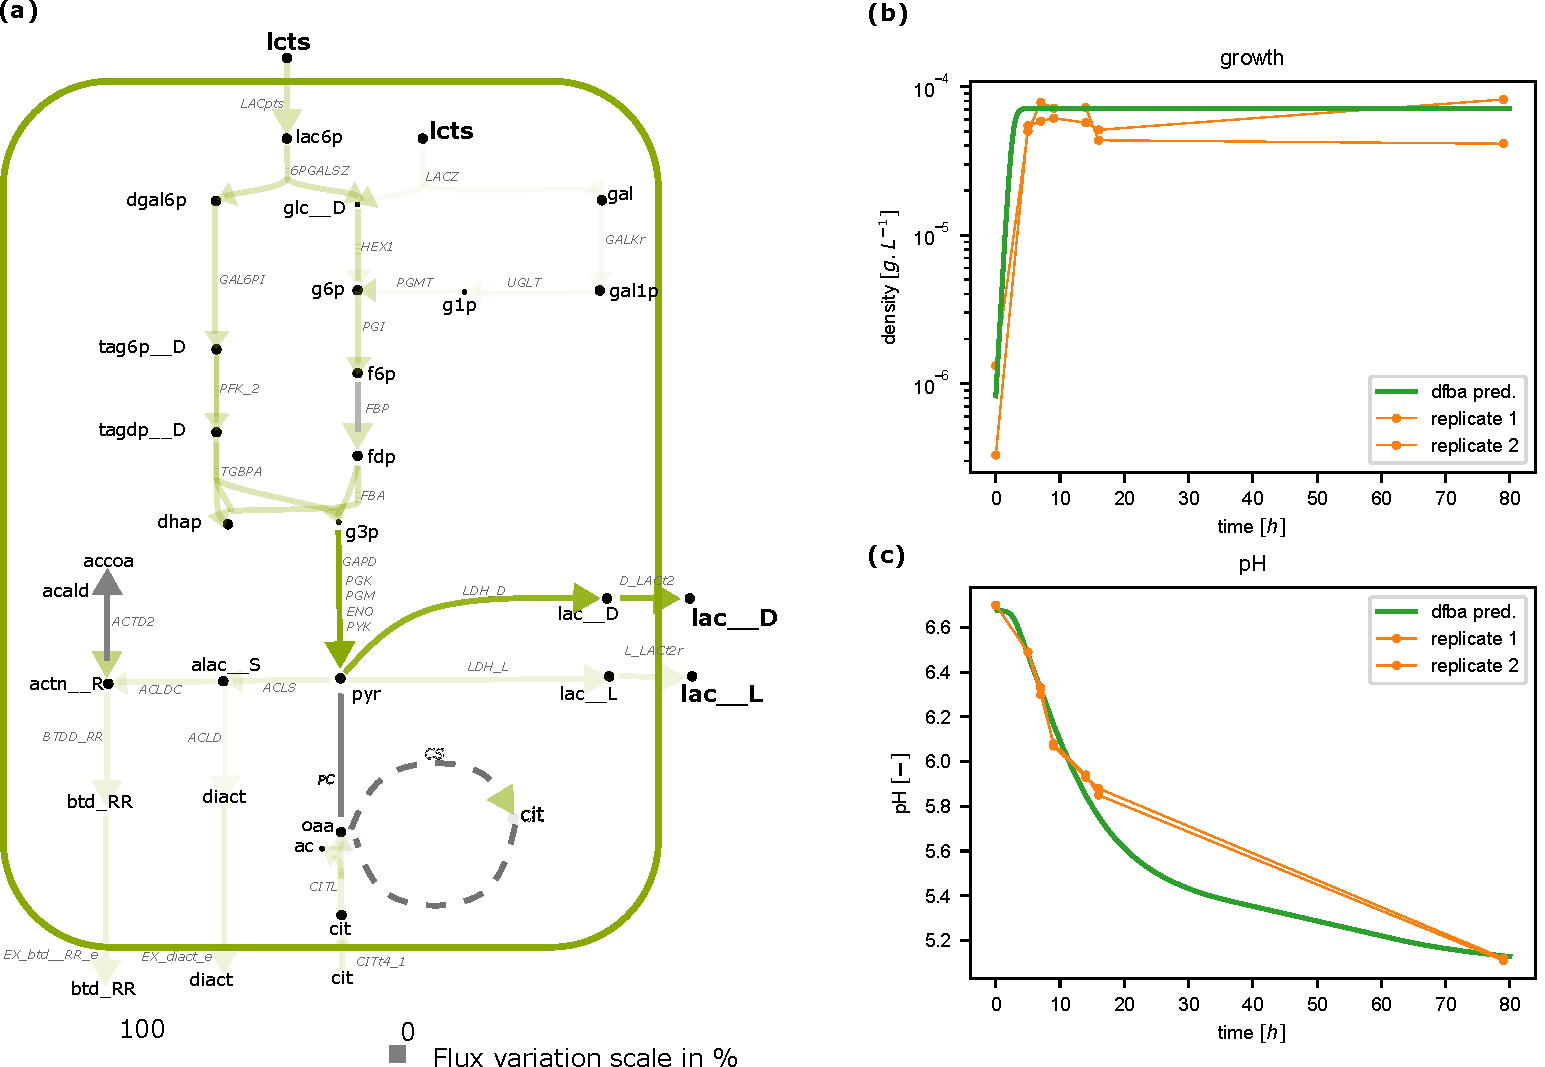
\includegraphics[width = 1\textwidth]{img/tango/FIG2_opt_explo_ll.pdf}
    \caption{\textbf{ Réseau métabolique de \lactis après calibration sur les données de culture pure.} (a) Représentation d'un FBA appliqué sur le métabolisme carboné central lors de l'inoculation de \lactis. L'échelle de couleur représente les valeurs de flux prédites par le FBA et normalisées par la plus haute valeur de flux prédites sur les voies métaboliques illustrées. (b) Simulation de la croissance de \lactis au cours du temps après inférence des paramètres dans le modèle (courbe verte) et d'après les données expérimentales (courbe orange, with $\pm 1/4$ log, which is the admitted range of precision for plating numbering). (c) Courbes de pH dans des conditions de culture pure simulé par le modèle (courbe verte) et issues des données expérimentales (croix orange , with standard deviation). La liste des métabolites et des réactions est répertoriée à la fin du chapitre à la section \ref{abbreviation-reac}}
    \label{dfba_metabolite_lactis}
\end{figure}

Contrairement à \lactis, le modèle métabolique de \plantarum semble avoir une préférence de production pour le lactate, montrant ainsi sa contribution à l'acidification du fromage. La voie de la glycolyse est active, ainsi que la consommation du lactose jusqu'à la production des deux formes du lactate. Nous remarquons également un flux de production de l'acide acétique par la voie de l'acétatekinase, contribuant plus faiblement à l'acidification (Fig. \ref{figure:metabolic_map_plantarum}). Les simulations dynamiques de \plantarum ont montré une activation des voies fermentaires hétérolactique et homolactique. Cependant à notre connaissance, la voie métabolique de la transkétolase, représentant la fermentation hétérolactique, est observée pour la première fois dans un contexte laitier. La consommation du citrate est connue pour être dépendante de la souche au sein de l'espèce \plantarum \citep{Palles1998}. Elle a été observée dans notre cas à travers la réaction de transport $FEDCabc$, conduisant à une augmentation de la quantité de pyruvate intracellulaire. \\

\begin{figure}[h!]
    \centering
    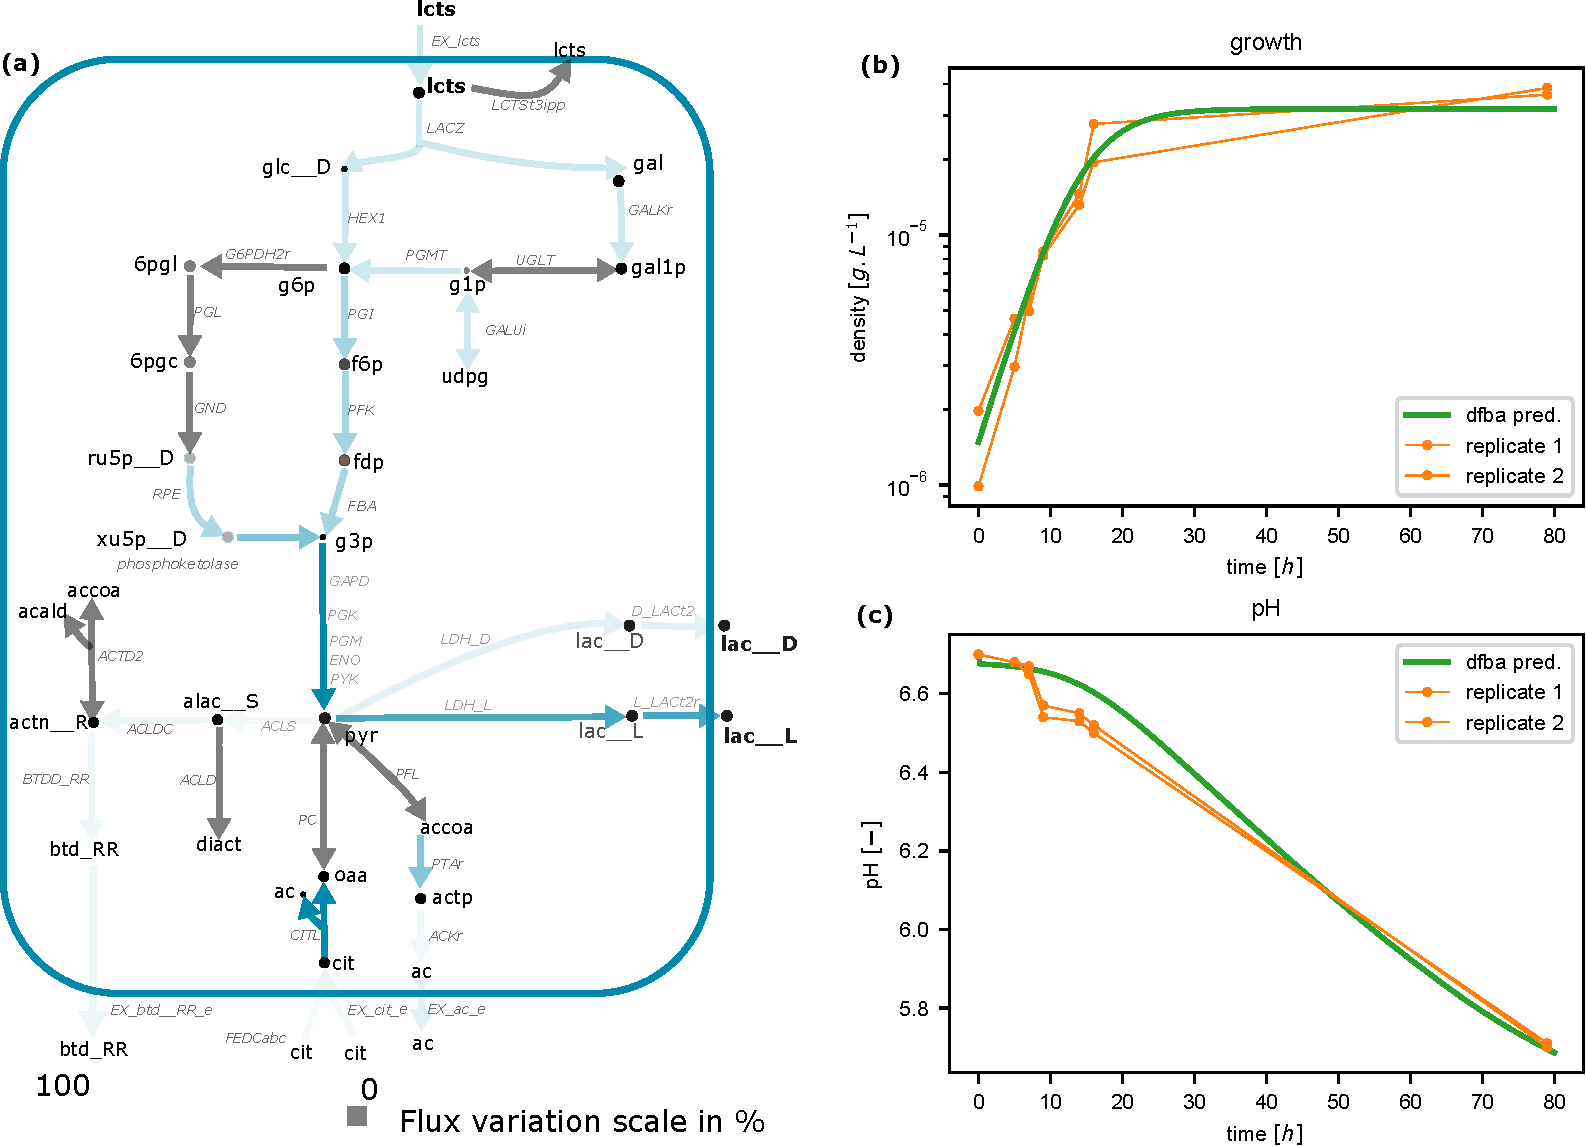
\includegraphics[width = 1\textwidth]{img/tango/FIG3_opt_explo_lp.pdf}
    \caption{\textbf{Réseau métabolique de \plantarum après calibration sur les données de culture pure.} (a) Représentation d'un FBA appliqué sur le métabolisme carboné central lors de l'inoculation de \plantarum. L'échelle de couleur représente les valeurs de flux prédites par le FBA et normalisées par la plus haute valeur de flux prédites sur les voies métaboliques illustrées. (b) Simulation de la croissance de \plantarum au cours du temps après inférence des paramètres dans le modèle (courbe verte) et d'après les données expérimentales (courbe orange, with $\pm 1/4$ log, which is the admitted range of precision for plating numbering). (c) Courbes de pH dans des conditions de culture pure simulé par le modèle (courbe verte) et issues des données expérimentales (croix orange , with standard deviation). La liste des métabolites et des réactions est répertoriée à la fin du chapitre à la section \ref{abbreviation-reac}}
    \label{dfba_metabolite_plant}
\end{figure}

 
Enfin, le modèle FBA de \freud consomme préférentiellement du lactose malgré la présence de l'acide lactique (Fig. \ref{dfba_metabolite_freud}a). Cependant, nous retrouvons une activation simultanée des cycles du TCA et de Wood-Werkman \citep{Deborde2000}, le premier permettant la régénération des sources de carbone nécessaires pour l'activation du second et ainsi, la production de propionate.

\begin{figure}[htpb!]
    \centering
    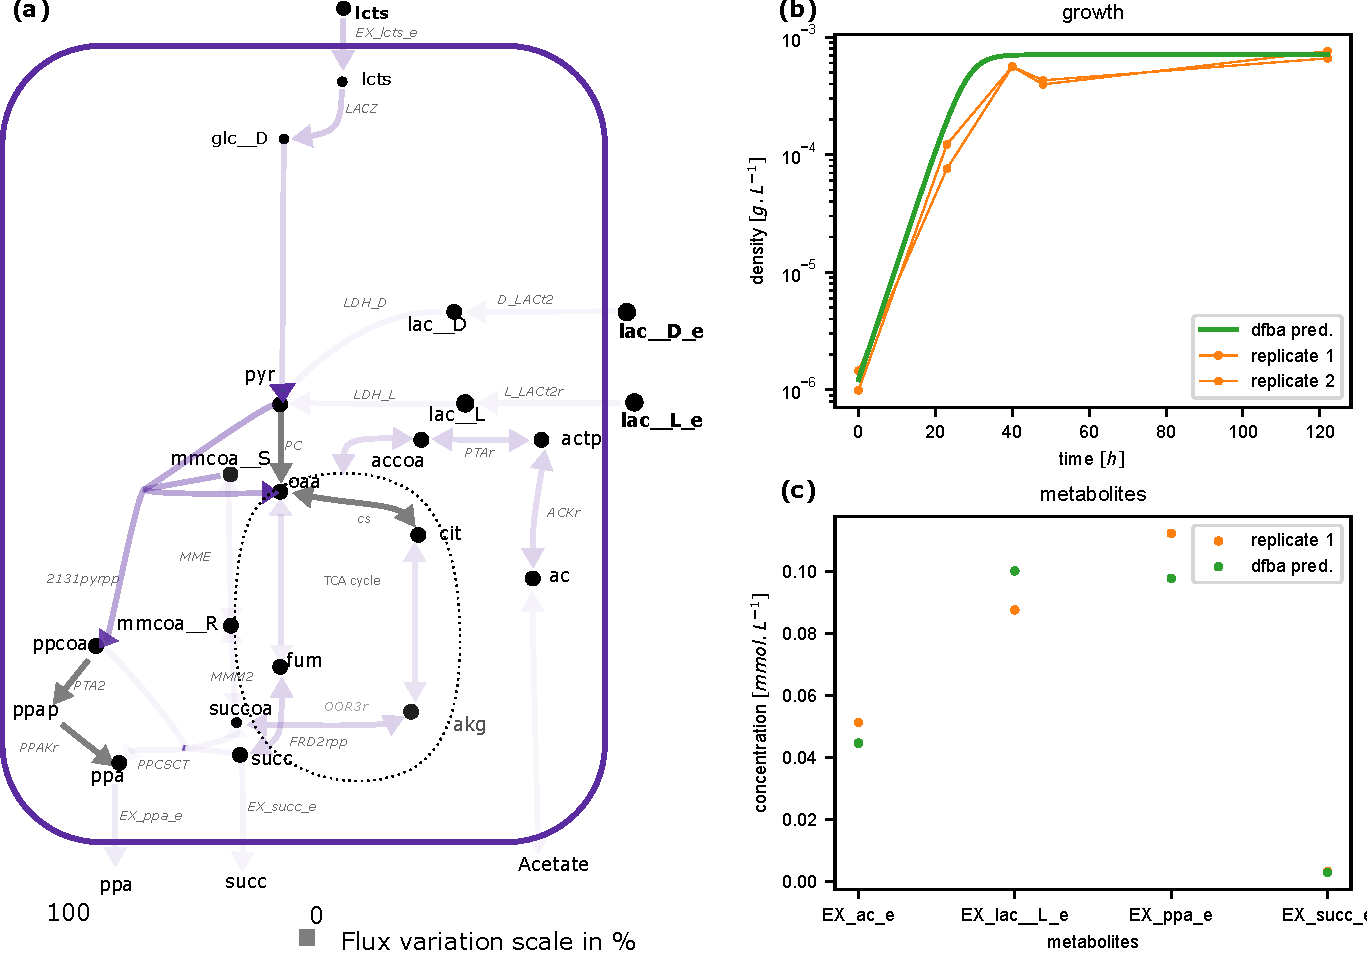
\includegraphics[width = 1\textwidth]{img/tango/FIG4_opt_explo_pf.pdf}
    \caption{\textbf{Réseau métabolique de \freud après calibration sur les données de culture pure.} (a) Représentation d'un FBA appliqué sur le métabolisme carboné central lors de l'inoculation de \freud. L'échelle de couleur représente les valeurs de flux prédites par le FBA et normalisées par la plus haute valeur de flux prédites sur les voies métaboliques illustrées. (b) Simulation de la croissance de \freud au cours du temps après inférence des paramètres dans le modèle (courbe verte) et d'après les données expérimentales (courbe orange, with $\pm 1/4$ log, which is the admitted range of precision for plating numbering). (c) Concentrations de lactate, acetate, propionate et succinate simulées (points verts) observées (croix en orange avec un écart-type) au temps final. La liste des métabolites et des réactions est répertoriée à la fin du chapitre à la section \ref{abbreviation-reac}
    }
    \label{dfba_metabolite_freud}
\end{figure}


Les sous figures (b) des Figures \ref{dfba_metabolite_lactis},\ref{dfba_metabolite_plant},\ref{dfba_metabolite_freud} montrent que les courbes de croissance simulées (en vert) sont fidèles aux données de croissances expérimentales de chaque souche microbienne. Concernant le pH, pour les sous figures~\ref{dfba_metabolite_lactis}, \ref{dfba_metabolite_plant} (c), nous avons observé que l'utilisation de la concentration du lactate dans une approximation du pH permet d'expliquer le pH observé lors des cultures pures de \lactis et \plantarum. Enfin, notre modèle métabolique de \freud retrouve les concentrations finales prédites par les expériences biologiques (Figure \ref{dfba_metabolite_freud}(c)). Afin de vérifier statistiquement que l'apprentissage de nos modèles est correct, nous avons représenté sur la figure Fig.~\ref{fig:qqplot} (a) les valeurs de croissance, de pH et de métabolites calculés par notre modèle et celles des données expérimentales. Nous observons une très bonne corrélation avec une valeur de $\text{R}^2$ = 0.99, montrant ainsi que nos modèles métaboliques individuels sont suffisamment bien ajustés. \\

\begin{figure}[h!]
    \centering
    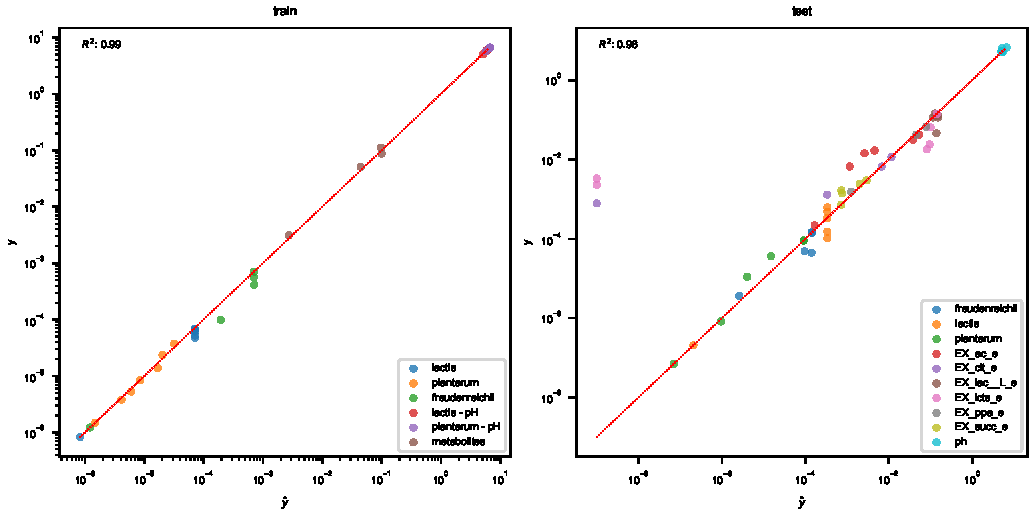
\includegraphics[width = 1\textwidth]{img/tango/qqplot.pdf}
    \caption{\textbf{Validation des prédictions après apprentissage.} Les valeurs simulées issues des modèles ($\hat{y}$) et celles des données expérimentales respectives ($y$) lors de la phase d'apprentissage sur les données de cultures pures (a) et lors de la phase de test en communauté (b). La couleur représente le type de la donnée et la bissectrice est affichée par une ligne en pointillée rouge. Le $R^2$ est calculé selon la formule suivante : $R^2 = 1 - \frac{\sum_i (y_i - \hat{y}_i)^2)}{\sum_i (y_i - \bar{y}_i)^2)}$ où $\bar{y}$ est la valeur moyenne de $y$. Nous pouvons observer une bonne capacité du modèle à prédire les concentrations.}
    \label{fig:qqplot}
\end{figure}

Nous venons de voir tout le processus d'itération statique et dynamique nécessaire pour obtenir des modèles métaboliques complets et des prédictions numériquement fiables. L'étape finale pour la construction d'un modèle numérique explicatif du fonctionnement de cette communauté fromagère est de passer à l'échelle en créant un modèle de communauté afin de prédire les croissances de chaque souche en communauté, et dans un deuxième temps, d'explorer les interactions bactériennes potentielles et les contributions de chaque souche pour la production et la consommation de métabolites.

\subsection{Simulations à l'échelle de la communauté}
En premier lieu, nous avons créé un modèle de communauté où chaque espèce maximise sa propre biomasse et avons utilisé les modèles calibrés sur les données de cultures pures pour construire ce modèle.
Nous avons ensuite ajusté la valeur du "quorum sensing", correspondant à la valeur à laquelle nous observons une phase plateau, de chaque modèle individuel en intégrant la valeur de "quorum sensing" des données expérimentales en co-culture (voir la Table \ref{com_data} et l'équation \ref{eq:logistic-growth} dans le but de reproduire le comportement métabolique de la communauté \textit{in silico} (voir eq.~\ref{eq:system_dynamics_b}-\ref{eq:system_dynamics_m}). Ce modèle de communauté n'a subi aucun processus de calibration sur les nouvelles données, c'est à dire, aucun paramètre basé sur la métabolomique ou sur les données de croissance en co-culture n'a été utilisé afin d'affiner les prédictions. Ces données vont en revanche être consacrées à la validation des prédictions du modèle.

Les simulations de la croissance, du pH et de la métabolomique du modèle de communauté ont correctement expliqué les valeurs expérimentales (Fig. \ref{dfba_community}(a)-(c), Table supplémantaire \ref{table:co-culture-data}). Nous avons remarqué cependant une légère surestimation de la croissance de \freud durant la phase exponentielle. Concernant la prédiction des concentrations de métabolites issus de la métabolomique, nous avons observé une consommation plus lente du lactose tandis que celle du citrate s'ajuste bien avec les données expérimentales. La production de lactate est légèrement sur-prédite durant la phase exponentielle résultant d'une sur-acidification du fromage durant les étapes de moulage et de démoulage. En revanche, la production d'acétate est sous-prédite durant les premières phases de la fabrication du fromage, mais le taux de production pendant la maturation est correctement modélisé. Les courbes du propionate, et dans une moindre mesure, celle du succinate sont prédites avec précision par le modèle suggérant que la production de composés organoleptiques par \freud est correctement capturée. De plus, les voies métaboliques activées en mono-cultures le sont également en co-culture (Figure \ref{fig:switch_metabolic_pathway}). Enfin, afin de valider statistiquement les prédictions du modèle en communauté, nous avons fait une régression entre les valeurs prédites par le modèle et celles des données, et nous observons un $\text{R}^2$ global de 0.98 pour cette étape de validation ( Figure \ref{fig:qqplot}, b). 

\begin{figure}[H]
    \centering
    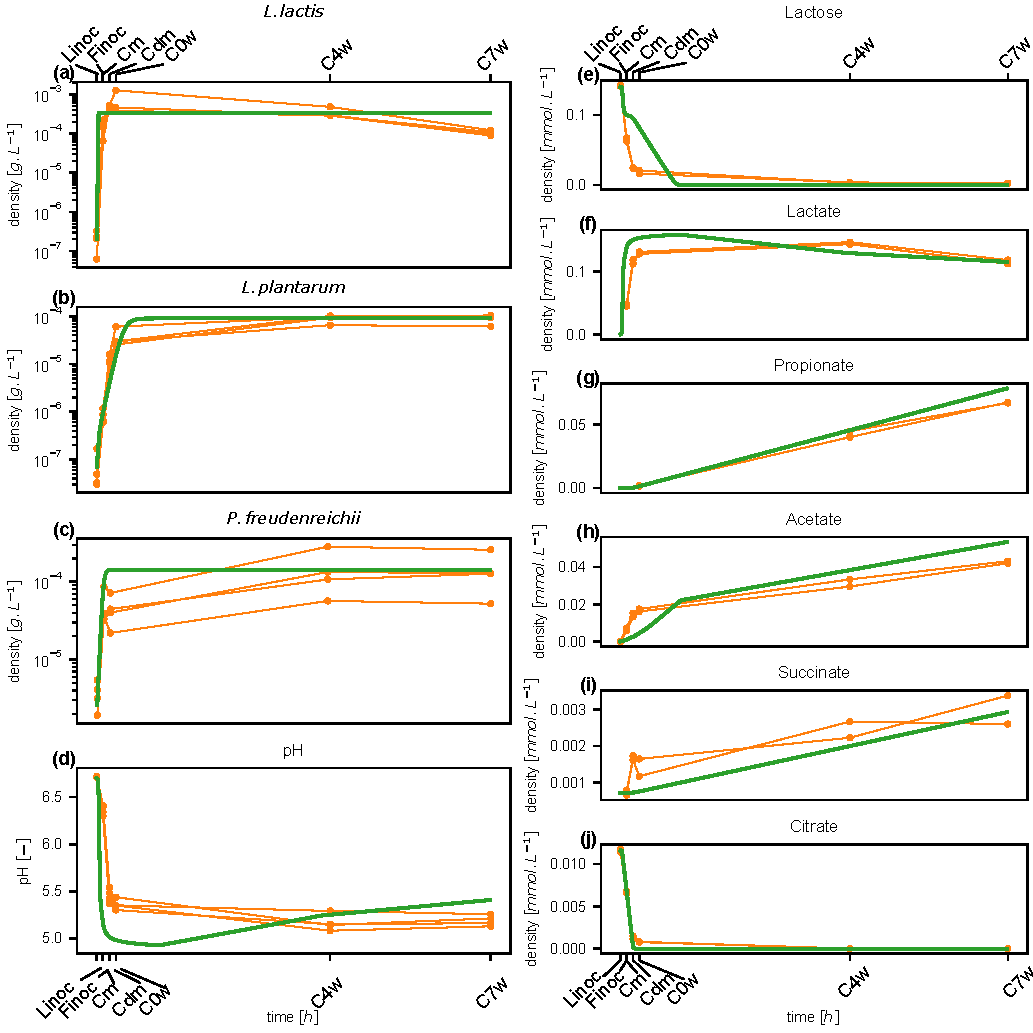
\includegraphics[width = 1.0\textwidth]{img/tango/Fig5.pdf}
    \caption{(a-c) Courbes de croissance de respectivement  \textit{L. lactis}, \textit{P. freudenreichii} and \textit{L. plantarum} calculées par le modèle (ligne verte) et celles observées expérimentalement (en orange). (d-j) Profil métabolique et du pH en condition de co-culture calculé par le modèle et expérimentalement observé. L'écart-type est représenté pour chaque point des données.  Abréviations: Linoc, innoculation des LAB (t = 0); Finoc, inoculation de \textit{P. freudenreichii}  (t = 18 hours); Cm, moulage (t = 19.5 hours); Cdm, démoulage (t = 40 hours); C0w, début d'affinage (t = 60 hours); C4w,4 semaines d'affinage (t = 732 hours); C7w, 7 semaines d'affinage (t = 1236 hours).}
    \label{dfba_community}
\end{figure}

\begin{figure}[H]
    \centering
    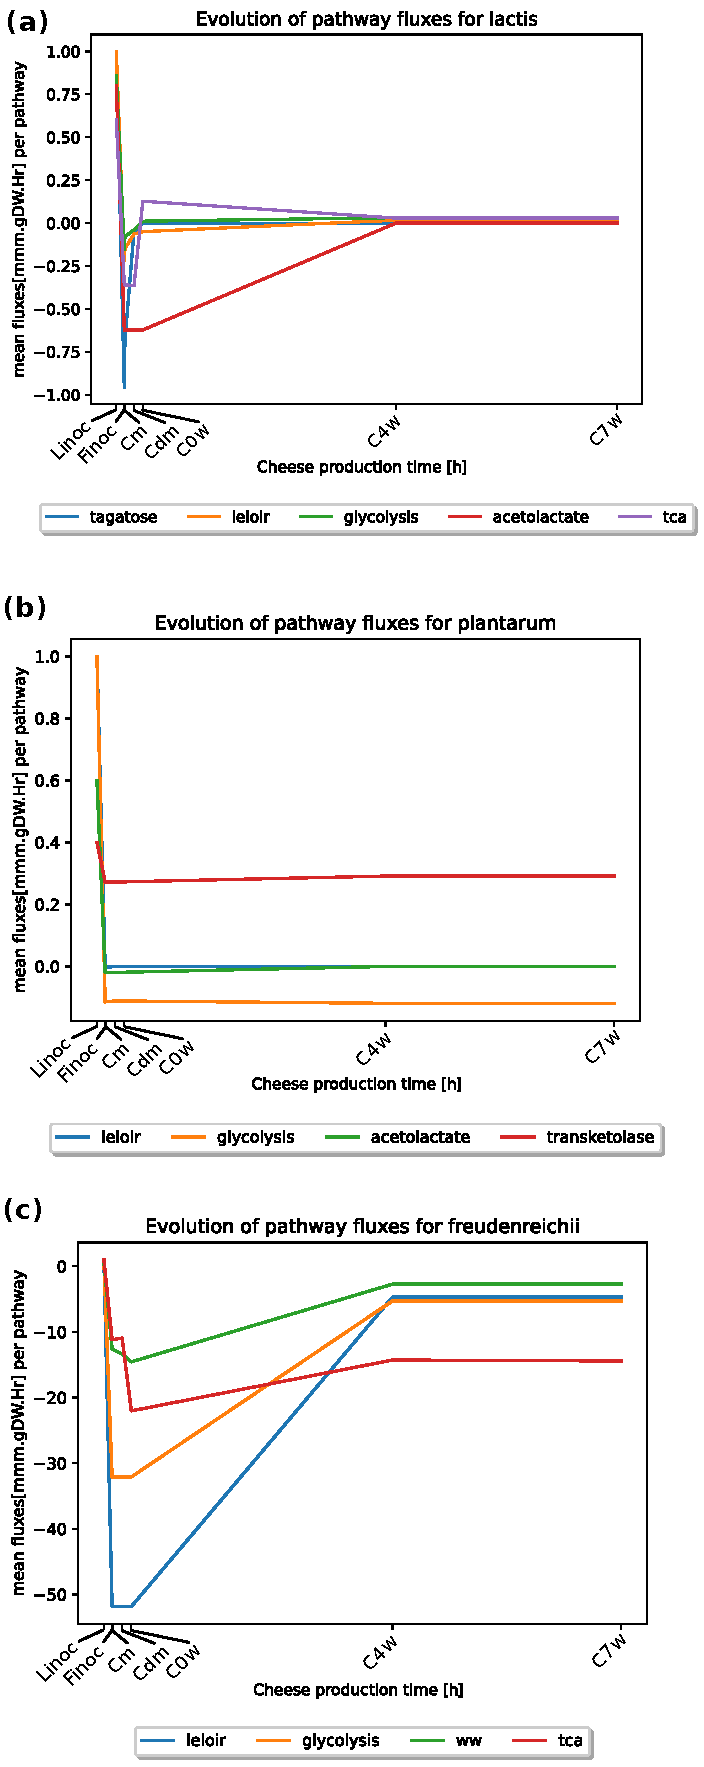
\includegraphics[width=0.5\textwidth]{img/tango/supp_fluxes_pathways.pdf}
    \caption{\textbf{Illustration du changement de voies métaboliques durant le processus de production du fromage.} Pour chaque bactérie nous avons lancé une simulation dynamique (dFBA) et les flux réactionnelles pour chaque voies métaboliques d'intérêt des figures \ref{figure:metabolic_map_lactis},\ref{figure:metabolic_map_plantarum},\ref{figure:metabolic_map_freud} on été retrouvé à l'incoculation de bactéries lactiques (Linoc, t=0 heure), de \freud (Finoc, t=18 heures), au moulage(t=19.5 heures), demoulage (Cdm, t=40heures), début de l'affinage (C0w, t=60 heures), après 4 (C4w, t=732 heures) et 7 (C7w, t=1236 heures) semaines d'affinage. Nous avons normalisés les flux par la valeur de flux lors de l'inoculum.}
    \label{fig:switch_metabolic_pathway}
\end{figure}

En somme, nous avons montré qu'utiliser uniquement des modèles métabolique curés et calibrés individuellement permet de retrouver les observations en communauté. Malgré les deux étapes itératives coûteuses en temps, l'interactivité entre modèle numérique et connaissance biologique \textit{a priori} permet d'obtenir des prédictions à l'échelle d'une communauté avec une bonne précision. Grâce à cette assurance, nous avons pu exploiter davantage le modèle de communauté du point de vue des interactions bactériennes possibles au sein de cette communauté. Dans les paragraphes suivant, nous déduirons dans un premier temps des interactions que notre approche numérique a pu mettre en évidence en analysant les flux relatifs et absolus de production et de consommation de métabolite par espèce. Dans un second temps, nous verrons ce que des outils sans connaissance \textit{a priori} peuvent découvrir.  \\

\subsection{Interactions bactériennes et exploration du modèle de communauté}

Notre modèle numérique de communauté peut révéler des interactions microbiennes du type syntrophiques, dans laquelle une espèce se nourrit des produits de l'autre, ou du type compétition pour un nutriment. Dans ce but, nous nous sommes focalisés sur la dynamique des flux des métabolites d'intérêt pour chaque espèce (Fig. \ref{fig:flux-contrib}, (a)) en calculant, à chaque pas de temps de la dynamique, et à l'échelle de la population, les flux d'échange $\mu_{i,j} b_i$ pour chaque métabolite $j$ et bactérie $i$ et les concentrations des métabolites associées. Concernant le lactose et le citrate, nous observons que \lactis les consomment très rapidement durant sa phase exponentielle Nous pouvons observer que \plantarum ne contribue pas ou peu à la consommation totale de ces métabolites suggérant ainsi que d'autres métabolites non suivis en dynamique sont utilisés pour la croissance de ce dernier, comme par exemple, les acides aminés. La croissance plus lente de \plantarum dans les premières heures du processus de production du fromage pourrait expliquer cette observation. En effet, on remarque que la régulation sur les bornes de consommation du lactose et du citrate sont mis en jeu lorsque la densité bactérienne de \plantarum est encore faible. De manière surprenante, nous observons que \freud termine la déplétion du lactose à la place de \plantarum au tout début de la phase d'affinage, bien que le lactate, source préférentielle de cette espèce, soit déjà produit, indiquant une ségrégation temporelle de l'utilisation de lactose, et une absence de compétition directe pour ce substrat.

\begin{figure}[H]  
    \centering
        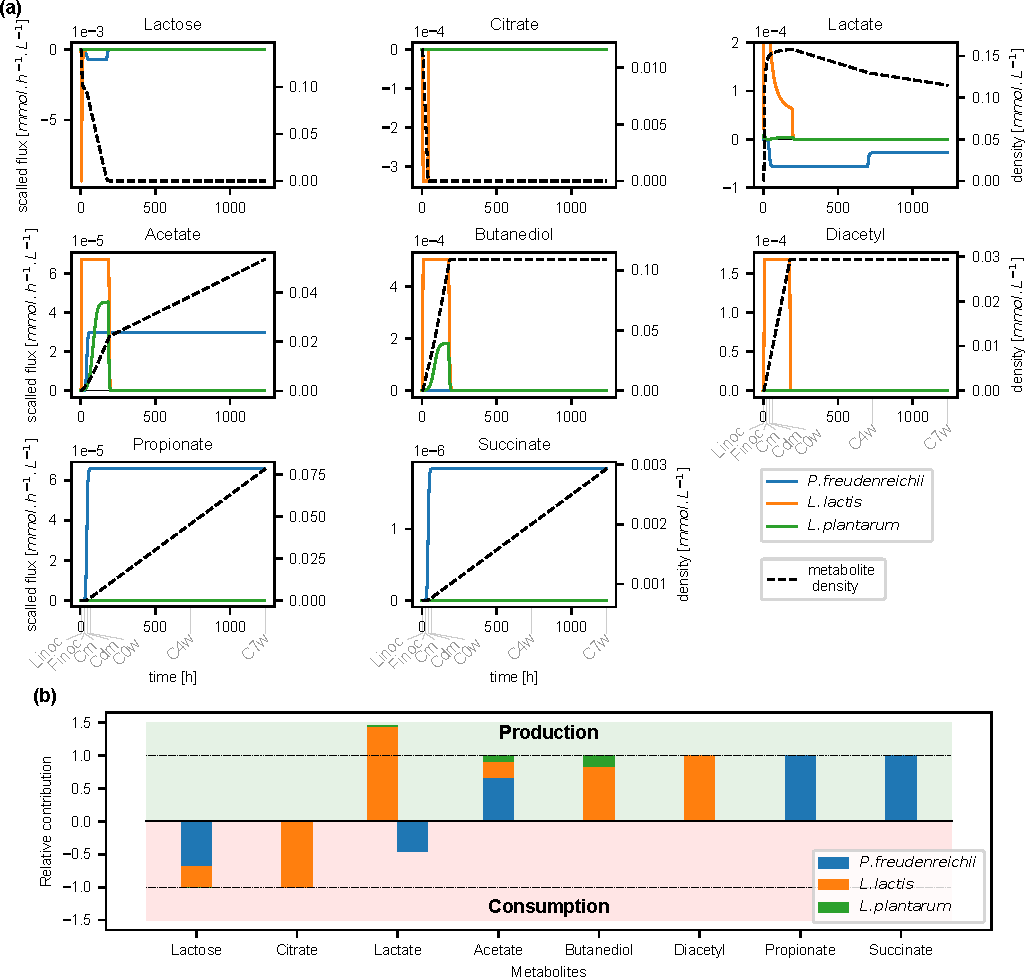
\includegraphics[width = 1.0\textwidth]{img/tango/Fig6.pdf}
        \caption{(a) \textbf{Flux dynamiques de consommation et de production de métabolites d'intérêts.} Nous representons pour chaque bactérie les flux dynamiques de consommation et de production de chaque métabolites que l'on en simulation (lignes coloriées). La dynamique de la concentration de ces mêmes métabolites dans le fromage est aussi représenté par les traits en pointillés. (b) \textbf{Contribution relative des bactéries dans le devenir des métabolites.} Nous avons calculé pour chaque souche sa contribution totale dans la consommation et la production de ces métabolites et intégré en temps par :$\int_0^t \mu_{i,j} b_i$ pour le métabolite $j$ et la bactérie $i$, voir eq.\ref{eq:system_dynamics_m}). Par la suite, nous avons normalisé le résultat par la somme des bactéries. La valeur 1 (resp. -1) représente la production (consommation) nette, \textit{i.e.}, la différence de concentration du métabolite à l'état final et initial (ligne en pointillé).  Abbreviations: Linoc, inoculation des bactéries lactiques (t = 0); Finoc, \textit{P. freudenreichii} inoculation (t = 18 hours); Cm, moulage (t = 19.5 hours); Cdm, Démoulage (t = 40 hours); C0w, début de l'affinage (t = 60 hours); C4w, 4 semaines d'affinage (t = 732 hours); C7w, 4 semaines d'affinage (t = 1236 hours).}
        \label{fig:flux-contrib}
    \end{figure}
    

La production de lactate étant corrélée avec la consommation de lactose, nous observons une très forte production par \lactis pendant 250 heures, correspondant à l'affinage dans le processus de fabrication du fromage. Malgré la plus faible croissance de \plantarum, ce dernier contribue peu à la production de lactate. Durant la phase de l'affinage, le lactate est consommé par \freud contribuant ainsi à l'augmentation du pH dans la communauté comme observé dans la Figure~\ref{dfba_community}~d. De façon surprenante, toutes les souches sont capables de produire l'acétate dans le milieu extracellulaire. \lactis est le contributeur majeur suivi par \plantarum jusqu'au temps t = 250 heures, temps à partir duquel la phase plateau commence. Ce schéma est retrouvé chez les bactéries lactiques intervenant également dans la production du butanediol \textit{via} la voie de l'acétolactate. Cependant, \freud continue de garder un taux de production constant d'acétate durant la maturation du fromage malgré la phase plateau atteinte. Enfin, le propionate et le succinate sont produits à taux constant par \freud durant tout le processus d'affinage et seule la souche de \lactis semble être capable de produire le diacétyle jusqu'au début de la période de l'affinage.\\

Afin d'obtenir la contribution en flux net de chaque souche au sein de ce consortium, nous avons intégré dans le temps la prédiction du FBA $\int_0^T \mu_{i,j}(t) b_i(t) dt$. Après normalisation de cet échange net par les échanges totaux au sein de la communauté (\textit{i.e.} la somme des échanges net de chaque individu), nous avons obtenu les contributions de chaque souche dans la production et la consommation de chaque métabolite (Fig. \ref{fig:flux-contrib}, (b)). Ces contributions confirment que le succinate et le propionate sont uniquement produits par \freud, alors que le diacétyle (production) et le citrate (consommation) sont métabolisés par \lactis. \plantarum contribue à la production du butanediol, bien que le principal producteur semble être \lactis. Dans une moindre mesure, \lactis contribue plus que \plantarum à la production de l'acétate dominée par \freud. En terme d'interactions bactériennes, on observe une syntrophie pour le lactate entre \lactis (producteur) et \freud (consommateur).\\

Nous avons démontré ci-dessus que capturer la complexité des processus métaboliques dans une communauté microbienne durant la fabrication de fromage requiert des considérations de la dynamique sous-jacente  du système. Nous nous demandions si l'application d'approches computationelles \textit{a priori} reposant sur les modèles métaboliques à l'échelle du génome peuvent mettre en avant de nouvelles interactions putatives entre les souches. A cette fin, nous avons utilisé deux méthodes basées sur les flux, SMETANA \citep{Zelezniak2015} et MiCOM \citep{diener2020}, et une approche qualitative basée sur le raisonnement, Metage2Metabo \citep{Belcour.2020} dans le but de suggérer de nouvelles complémentarités métaboliques au sein du consortium.

Les approches quantitative, MiCOM et SMETANA, ont mis en avant respectivement 14 et 25 métabolites échangés (Table\ref{table:exchangeable-metabolites-MICOM} et \ref{table:exchangeable-metabolites-smetana}), alors que l'approche par raisonnement, Metage2Metabo, identifie 11 métabolites qui ne peuvent pas être produits par une espèce sans interactions dans la communauté (Table \ref{table:added-value-M2M}). 

Une première observation est qu'un nombre assez important (11) de métabolites sont communs dans les prédictions des composés échangeables de SMETANA et MiCOM: lactate, qui est aussi prédit dans le modèle dynamique, phénylalanine, serine, malate, succinate, xanthine, H${_2}$S,2-ketoglutarate, glycolate et acetaldehyde. Les autres composés échangés prédits incluent principalement des acides aminés (isoleucine, proline, glycine, alanine). Pour chaque composé mis en avant par SMETANA nous avons utilisé les données méta-transcriptomiques dans le but d'évaluer la validité des interactions les plus plausibles selon le score SMETANA. Le H${_2}$S est prédit comme produit de \lactis et \plantarum au bénéfice de \freud, le ribose est produit par \lactis et \plantarum et consommé par \freud, le glycerol produit par les bacteries lactiques et consommé par \freud) et enfin la phénylalanine produite uniquement par \plantarum et consommée par \freud. Pour chacun de ces métabolites prédits comme échangés, nous avons vérifié l'expression des gènes associés à la production de ces métabolites chez les espèces donneuses, et à la consommation de ces métabolites chez les espèces receveuses (voir methodes et Figure \ref{fig:heatmap_metaT}). Les résultats suggèrent que les interactions pour H${_2}$S, ribose et le glycerol sont plausibles à plusieurs étapes de la fabrication du fromage. A l'inverse, alors que les données d'expression de gènes montrent que les voies métaboliques de la consommation de la phénylalanine sont fortement exprimées chez \freud, leur production par \plantarum ne l'est pas, suggérant que cette interaction semble être moins recevable. 


\begin{table}[H]
\centering
\begin{adjustbox}{width=\textwidth}
\begin{tabular}{|c|c|c|c|c|c|}
\hline
ID Bigg & ID Metacyc & Nom & Ontologie Metacyc&fluxes d'export & fluxes d'import\\
\hline
acald\_e	& ACETALD &	acetaldéhylde & Aldehydes-Or-Ketones, Aldehydes	& Pf; Ll &	Lp \\
akg\_e &	2-KETOGLUTARATE	& 2-oxoglutarate &	Acids, Organic-Acids	& Pf &	Lp \\
ala\_\_D\_e &	D-ALANINE &	D-ALANINE &	All-Amino-Acids, Acids, Amino-Acids, Organic-Acids	& Pf; Lp &	Ll \\
ala\_\_L\_e	& L-ALPHA-ALANINE &	L-ALPHA-ALANINE &	All-Amino-Acids, Acids, Amino-Acids, Organic-Acids	& Pf; Lp	& Ll \\
co2\_e &	CARBON-DIOXIDE	& CARBON-DIOXIDE	& Others, Others	& Pf; Ll &	Lp \\
coa\_e &	CO-A &	co enzyme A &	Groups, Others	& Pf; Ll	& Lp \\
fe2\_e	& FE+2	& Fe2+&	Ions, Inorganic-Ions, Cations &	Lp	& Pf; Ll \\
gly\_e	& GLY	& Glycine	& All-Amino-Acids, Acids, Amino-Acids, Organic-Acids &	Lp &	Pf; Ll \\
glyclt\_e &	GLYCOLATE &	GLYCOLATE	& Acids, Organic-Acids	& Pf &	Lp \\
gthox\_e &	OXIDIZED-GLUTATHIONE &	glutathione disulfide	& ORGANOSULFUR, All-Glutathiones &	Lp &	Ll \\
gthrd\_e	& GLUTATHIONE &	glutathione	& ORGANOSULFUR, All-Glutathiones, Thiols	& Ll	& Lp \\
h2o2\_e &	HYDROGEN-PEROXIDE &	hydrogen peroxide &	Peroxides, Others	& Ll &	Lp \\
h2o\_e	& WATER	& H2O	& Pseudo-Compounds, Others &	Pf; Ll	& Lp \\
h2s\_e	& HS	& hydrogen sulfide &	Ions, Anions, Inorganic-Ions	& Ll	& Lp; Pf \\
ile\_\_L\_e &	ILE &	isoleucine &	All-Amino-Acids, Acids, Amino-Acids, Organic-Acids &	Lp	& Pf; Ll \\
lac\_\_D\_e &	D-LACTATE &	d-lactate &	Acids, Organic-Acids	& Pf &	Ll; Lp \\
lac\_\_L\_e &	L-LACTATE &	l-lactate &	Acids, Organic-Acids &	Ll	& Lp; Pf \\
mal\_\_L\_e &	MAL	& malate &	Acids, Organic-Acids	& Pf; Lp &	Ll \\
nh4\_e &	AMMONIUM &	ammonium &	Ions, Inorganic-Ions, Cations	& Lp	& Pf; Ll \\
phe\_\_L\_e &	PHE &	phenylalanine &	Aromatics, All-Amino-Acids, Acids, Amino-Acids, Organic-Acids, Organic-aromatic-compounds &	Pf	& Lp \\
pro\_\_L\_e &	PRO &	proline &	All-Amino-Acids, Acids, Amino-Acids, Organic-Acids &	Ll	& Pf \\
ser\_\_D\_e &	D-SERINE &	serine	& All-Amino-Acids, Acids, Amino-Acids, Organic-Acids &	Ll	& Lp; Pf \\
ser\_\_L\_e &	SER	& serine &	All-Amino-Acids, Acids, Amino-Acids, Organic-Acids &	Ll &	Lp; Pf \\
succ\_e &	SUC	& succinate	& Acids, Organic-Acids &	Ll &	Pf \\
xan\_e &	XANTHINE &	xanthine &	Others, Others &	Ll	& Lp; Pf \\
 \hline
\end{tabular}
\end{adjustbox}
\caption{\textbf{Métabolites échangeable sur la communauté du fromage identifiés par MICOM} Abréviations: Ll, \lactis; Lp, \plantarum, Pf, \freud}
\label{table:exchangeable-metabolites-MICOM}
\end{table}

\begin{table}[H]
\centering
\begin{adjustbox}{width=\textwidth}
\begin{tabular}{|c|c|c|c|c|c|}
\hline
ID Bigg & ID Metacyc & Nom & Ontologie Metacyc &fluxes d'export & fluxes d'import\\
\hline
acald\_e	& ACETALD	& acetaldéhylde	& Aldehydes-Or-Ketones, Aldehydes & \multicolumn{1}{c|}{{\begin{tabular}[c]{@{}l@{}}Pf \\ Pf \\ Lp \\ Ll \end{tabular}}}
& \multicolumn{1}{c|}{{\begin{tabular}[c]{@{}l@{}}Ll \\ Lp \\ Ll \\ Lp \end{tabular}}} \\
\hline
akg\_e &	2-KETOGLUTARATE	& 2-oxoglutarate &	Acids, Organic-Acids &\multicolumn{1}{c|}{{\begin{tabular}[c]{@{}l@{}} Lp \\ Pf  \end{tabular}}}
& \multicolumn{1}{c|}{{\begin{tabular}[c]{@{}l@{}} Pf \\ Lp \end{tabular}}} \\
\hline
fum\_e &	FUM	& fumarate &	Acids, Organic-Acids &\multicolumn{1}{c|}{{\begin{tabular}[c]{@{}l@{}}Pf \end{tabular}}}
& \multicolumn{1}{c|}{{\begin{tabular}[c]{@{}l@{}}Lp \end{tabular}}} \\
\hline
glyc\_e &	GLYCEROL &	GLYCEROL &	Alcohols, All-Carbohydrates, Sugar-alcohols, Carbohydrates &\multicolumn{1}{c|}{{\begin{tabular}[c]{@{}l@{}}Lp \\ Ll \\ Ll \end{tabular}}}
& \multicolumn{1}{c|}{{\begin{tabular}[c]{@{}l@{}}Pf \\ Pf \\ Lp \end{tabular}}} \\
\hline
glyclt\_e &	GLYCOLATE &	GLYCOLATE &	Acids, Organic-Acids &\multicolumn{1}{c|}{{\begin{tabular}[c]{@{}l@{}} Lp \end{tabular}}}
& \multicolumn{1}{c|}{{\begin{tabular}[c]{@{}l@{}} Pf \end{tabular}}} \\
\hline
h2s\_e	& HS	& hydrogen sulfide &	Ions, Anions, Inorganic-Ions &\multicolumn{1}{c|}{{\begin{tabular}[c|]{@{}l@{}}Lp \\ Pf \\ Ll \end{tabular}}}
& \multicolumn{1}{c|}{{\begin{tabular}[c]{@{}l@{}}Pf \\ Lp \\ Lp \end{tabular}}} \\
\hline
lac\_\_D\_e &	D-LACTATE	& d-lactate &	Acids, Organic-Acids &\multicolumn{1}{c|}{{\begin{tabular}[c]{@{}l@{}}Pf \\ Ll \end{tabular}}}
& \multicolumn{1}{c|}{{\begin{tabular}[c]{@{}l@{}}Lp \\ Lp \end{tabular}}} \\
\hline
lac\_\_L\_e &	L-LACTATE &	l-lactate &	Acids, Organic-Acids &\multicolumn{1}{c|}{{\begin{tabular}[c]{@{}l@{}} Ll \end{tabular}}}
& \multicolumn{1}{c|}{{\begin{tabular}[c]{@{}l@{}}Lp \end{tabular}}} \\
\hline
mal\_\_L\_e &	MAL	& malate &	Acids, Organic-Acids &\multicolumn{1}{c|}{{\begin{tabular}[c]{@{}l@{}}Pf \\ Lp \\ Pf \\ Ll \end{tabular}}}
& \multicolumn{1}{c|}{{\begin{tabular}[c]{@{}l@{}} Ll \\ Ll \\ Lp \\ Lp \end{tabular}}} \\
\hline
phe\_\_L\_e &	PHE	& phenylalanine &	\multicolumn{1}{c|}{{\begin{tabular}[c]{@{}l@{}} Aromatics, All-Amino-Acids, Acids, Amino-Acids \\Organic-Acids, Organic-aromatic-compounds \end{tabular}}}   &\multicolumn{1}{c|}{{\begin{tabular}[c]{@{}l@{}}Lp  \end{tabular}}}
& \multicolumn{1}{c|}{{\begin{tabular}[c]{@{}l@{}}Pf \end{tabular}}} \\
\hline
rib\_\_D\_e &	D-Ribopyranose &	D-Ribopyranose &	Aldehydes-Or-Ketones, All-Carbohydrates, Aldehydes, Carbohydrates &\multicolumn{1}{c|}{{\begin{tabular}[c]{@{}l@{}}Ll \\ Lp \\ Pf \\ Ll \end{tabular}}}
& \multicolumn{1}{c|}{{\begin{tabular}[c]{@{}l@{}}Pf \\ Pf \\ Lp \\ Lp \end{tabular}}} \\
\hline
ser\_\_D\_e	& D-SERINE	& serine &	All-Amino-Acids, Acids, Amino-Acids, Organic-Acids &\multicolumn{1}{c|}{{\begin{tabular}[c]{@{}l@{}}Ll \\ Lp
 \\ Pf \\ Lp \\ Pf \\ Ll\end{tabular}}}
& \multicolumn{1}{c|}{{\begin{tabular}[c]{@{}l@{}} Pf \\ Pf \\ Ll \\ Ll \\ Lp \\ Lp \end{tabular}}} \\
\hline
succ\_e &	SUC &	succinate &	Acids, Organic-Acids &\multicolumn{1}{c|}{{\begin{tabular}[c]{@{}l@{}}Ll \\ Lp \end{tabular}}}
& \multicolumn{1}{c|}{{\begin{tabular}[c]{@{}l@{}}Pf \\ Pf   \end{tabular}}} \\
\hline
xan\_e &	XANTHINE &	xanthine &	Others, Others &\multicolumn{1}{c|}{{\begin{tabular}[c]{@{}l@{}}Ll \\ Lp \end{tabular}}}
& \multicolumn{1}{c|}{{\begin{tabular}[c]{@{}l@{}}Pf \\ Pf   \end{tabular}}} \\
\hline
\end{tabular}
\end{adjustbox}
\caption{\textbf{Métabolites échangeable sur la communauté du fromage identifiés par SMETANA.} Abréviations: Ll, \lactis; Lp, \plantarum, Pf, \freud}
\label{table:exchangeable-metabolites-smetana}
\end{table}

\begin{figure}[H]
    \centering
    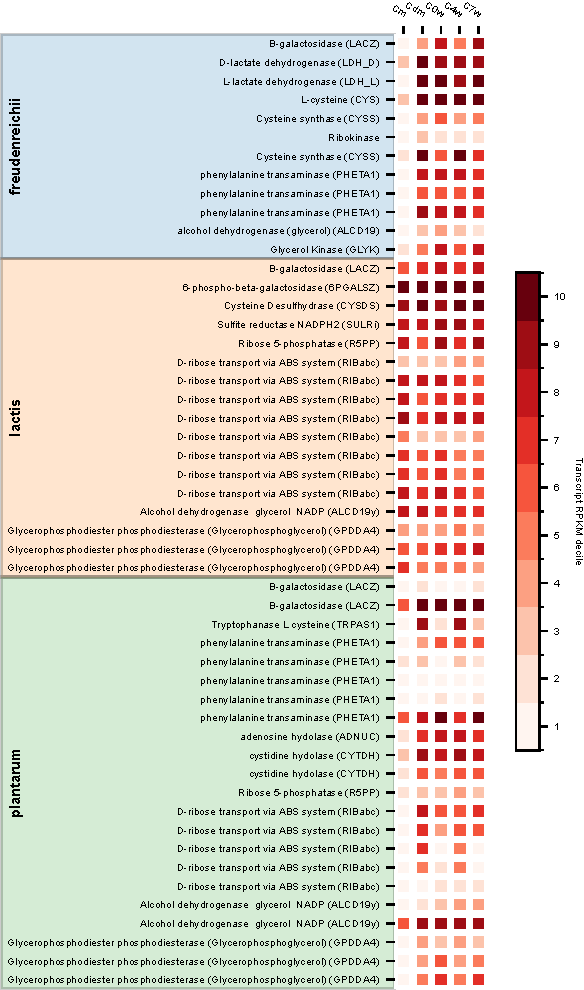
\includegraphics[width = 0.6\textwidth]{img/tango/FigS2_heatmap.pdf}
    \caption{\textbf{Expression des genes des données métatranscriptomiques} Cette carte thermique affiche le décile du nombre de RPKM de transcrits de gènes à un moment donné (colonnes) et dans un micro-organisme donné (les zones colorées indiquent à quelle bactérie le gène appartient). Les déciles ont ensuite été codés par couleur, des déciles les plus élevés (rouge foncé, expression la plus élevée dans ce micro-organisme à ce moment précis) aux déciles les plus bas (rouge clair, faible expression). Les gènes affichés ont été sélectionnés manuellement à partir de la liste des interactions possibles établie par SMETANA : pour un métabolite d'interaction sélectionné, les gènes impliqués dans la production (chez le donneur) et dans la consommation (chez le receveur) ont été retenus pour l'analyse. Les métabolites d'interaction sélectionnés sont le $H2S$, le ribose et la phénylalanine. En outre, les gènes impliqués dans la consommation de lactose ont été ajoutés à cette liste. Abbréviations: Cm, moulage (t = 19.5 hours); Cdm, démoulage (t = 40 hours); C0w, début de l'affinage (t = 60 hours); C4w, 4 semaines d'affinage (t = 732 hours); C7w, 7 semaines d'affinage (t = 1236 hours). }
    \label{fig:heatmap_metaT}
\end{figure}

Enfin, l'ensemble des métabolites dont la production est prédite par Metage2Metabo comme nécessitant des interactions dans la communauté inclut divers acides gras, comme le benzyl-Coa, le glyceraldehyde et la xanthosine, indiquant une complementarité métabolique entre les souches.



\begin{table}[H]
\centering
\begin{adjustbox}{width=\textwidth}
\begin{tabular}{|c|c|c|c|}
\hline
ID Bigg & ID Metacyc & Nom & Ontologie Metacyc  \\
\hline
galt1p&	D-galactose-1-phosphate&	a D-galactopyranose 1-phosphate	&All-Carbohydrates,Carbohydrates\\
benzcoa&	BENZOYLCOA&	benzoyl-CoA&	Esters,Thioesters\\
xtsn&	XANTHOSINE&	XANTHOSINE	&\begin{minipage}[t]{0.8\linewidth}Organic-heterocyclic-compound,All-Nucleosides,Nitrogen-Molecular-Entities,Organic-heteromonocyclic-compounds,Organic-Heteropolycyclic-Compounds,Organonitrogen-Compounds,Nucleosides\end{minipage}\\
glyald&	GLYCERALD&	glyceraldehyde	&Aldehydes-Or-Ketones,All-Carbohydrates,Aldehydes,Carbohydrates\\
3hocoa&	ø	&	ø	&	ø\\
3hhdcoa	&CPD0-2232	&(S)-3-hydroxyhexadecanoyl-CoA	&Thioesters,Esters\\
3hdcoa&	CPD0-2244	&(S)-3-hydroxydecanoyl-CoA	&Thioesters,Esters\\
3odcoa&	CPD0-2123&	3-oxodecanoyl-CoA	&Thioesters,Esters\\
3hhcoa&	OH-HEXANOYL-COA	&(S)-3-hydroxyhexanoyl-CoA&	Thioesters,Esters\\
udcpp&	UNDECAPRENYL-P	&all-trans-undecaprenyl phosphate	&Lipids,Polyisoprenoids\\
3oocoa&	CPD0-2106&	3-oxooctanoyl-CoA	&Thioesters,Esters\\
 \hline
\end{tabular}
\end{adjustbox}
\caption{\textbf{Liste de métabolites prédits par Metage2Metabo comme étant productibles uniquement par coopération métabolique}}
\label{table:added-value-M2M}
\end{table}

\section{Discussion et Conclusion}

Nous avons fourni un modèle numérique du métabolisme bactérien décrivant du point de vue métabolique, le processus de fabrication de fromage. En utilisant les modèles métaboliques de trois souches bactériennes inoculées et des données omiques, nous avons reproduit, avec précision, les motifs de production de métabolites ainsi que la dynamique des populations bactériennes. En nous reposant sur les conditions expérimentales de cultures pures pour calibrer les modèles métaboliques individuels avec peu de paramètres pour chacun, limitant ainsi le sur apprentissage du modèle durant les simulations communautaires. Une originalité du modèle est sa capacité à prédire les dynamiques sur tout le procédé de fabrication du fromage (sept semaines). Notre travail a généré des hypothèses sur les voies métaboliques mises en jeu dans le lait, ainsi que la contribution de chaque souche bactérienne dans la consommation de nutriments et la productibilité de composé organoleptiques. \\

La connaissance des microbiologistes, de la littérature scientifique et des données multi-omiques étaient nécessaires pour accomplir des modèles métaboliques à l'échelle du génome et des simulations dynamiques de qualité. Le métabolisme carboné central des bactéries lactiques produit principalement l'acide lactique à partir de la dégradation du lactose \textit{via} les voies métaboliques de la glycolyse, du tagatose et de Leloir \citep{Widyastuti2014,VanRooijen1991,Kleerebezem2003}. Pour la première fois, l'utilisation du citrate et de la fermentation hétérolactique ont été observé dans le modèle curé de \plantarum en lait. La vérification de modèle métabolique individuel et de l'activation des différentes voies métaboliques décrites plus haut représentait ainsi une étape importante pour valider les modèles, permettant la reproduction d'activités enzymatiques observées dans \citep{Quatravaux2006,Carroll1999}. La bactérie propionique \freud convertit le lactose, et préférentiellement le lactate en propionate d'après \citep{Loux2015,Thierry2011,Borghei2021}. Nous avons ajouté l'enzyme propionyl-CoA:succinate Coa transferase (2.8.3.-) pour compléter le cycle de Wood-Werkman, et ainsi assurer la production de propionate.

Dans \citep{Ozcan.2020}, les paramètres individuels de calibration pour chaque nutriment du milieu de culture sont imposés dans le but d'expliquer la métabolomique à l'échelle de l'espèce, et de prédire les composés de la métabolomique à l'échelle de la communauté. De plus, une nouvelle étape d'optimisation à l'échelle de la communauté a été faite afin d'affiner leur prédiction. Nous avons implémenté un modèle FBA dynamique en se basant sur \citep{Mahadevan.2002}, qui a utilisé des paramètres de calibration spécifiques aux souche pour prédire la croissance, le pH et les concentrations métaboliques. Pour éviter le sur apprentissage du modèle, nous avons réduit le nombre de paramètres inférés pour chaque bactérie. Seulement deux paramètres ont été gardés pour la régulation du pH pour les bactéries lactiques et un paramètre se focalisant sur les croissances de \plantarum et \freud. Des calibrations additionnelles ont été menées pour \freud sans aucune optimisation mathématique supplémentaire, en calculant la valeur de la borne supérieure des métabolites dosés en monoculture. Ainsi, nos paramètres ne sont pas propres à chaque nutriment et nous n'avons effectué aucune optimisation à l'échelle de la communauté.\\

Le modèle de co-culture a donné des indices sur le comportement de la communauté pendant la fabrication du fromage et a suggéré temporellement la contribution de chaque espèce impliquée dans la production des composés organoleptiques. Il est montré que la production de propionate peut être attribuée uniquement à \freud, comme indiqué dans \citep{Cao2021}, et que le diacétyl semble être seulement produit par \lactis. D'après le modèle de communauté, le butanediol a été produit pendant l'étape du moulage et au début de l'affinage par à la fois, \lactis et \plantarum, comme observé dans les modèles de monocultures respectifs. L'acétate est produit précocement jusqu'au début de l'affinage par les 3 espèces, puis, \freud, responsable de la majeure partie de production de l'acétate, semble le produire à flux constant jusqu'à la fin de la fabrication de fromage. Concernant l'utilisation des sources de carbone, alors que \plantarum possède les voies métaboliques de dégradation du lactose et du citrate, qui sont complètement activées dans le modèle en monoculture, il apparaît que ces voies métaboliques sont fortement sous régulés en co-culture et \plantarum ne semble plus être capable de métaboliser le citrate. Lors de la mise en culture avec \lactis, \plantarum atteint son efficacité métabolique maximale après la phase exponentielle de \lactis comme ce dernier a la plus faible vitesse de croissance. Étant donné que \lactis pousse principalement sur le lactose en produisant du lactate, sa phase exponentielle est associée à une forte acidification de milieu, réprimant probablement le métabolisme de \plantarum (voir equation sur la régulation du pH sur les bactéries lactiques). \plantarum peut utiliser des acides aminés ou d'autres métabolites non suivis par le modèle dynamique permettant sa croissance. Pour explorer cette piste, nous avons utilisé des outils dans le but d'identifier des interactions bactériennes en dehors de l'ensemble des composés suivis par le modèle dynamique en co-culture. Nous avons remarqué que parmi les possibles interactions, la famille des acides aminés était bien représentée.\\

Dans le modèle de co-culture, \freud garde son métabolisme activé  dans la dernière phase de production d'un fromage : l'affinage. Ce métabolisme est reflété par la consommation de lactate durant tout l'affinage, et le relargage de composés organoleptiques à flux constant (Figure \ref{fig:flux-contrib}). Ce comportement est cohérent avec les capacités métaboliques connues de \freud et avec les données métabolomiques obtenues expérimentalement. Dans le modèle, \freud consomme aussi le lactose restant après la croissance de \lactis. En effet, durant sa phase exponentielle, \lactis métabolise principalement le lactose, produisant fortement du lactate et réduisant le pH. La réduction du pH inhibe l'absorption du lactose dans les deux bactéries lactiques, et donc stoppant la consommation de lactose par les \textit{Lactobacilli}. Comme le lactose reste dans le milieu de culture et que \freud est l'unique bactérie capable de l'utiliser, il épuise donc le lactose encore présent. Dans les données métatranscriptomiques, le gène LACZ est fortement activé par \freud durant l'affinage confirmant la dégradation du lactose par cette souche après l'acidification (Figure \ref{fig:heatmap_metaT}) 


Ce chapitre a révélé comment le processus itératif, la combinaison d'expertise biologique, de données hétérogènes et de la modélisation métabolique permet d'obtenir des prédictions précises sur les mécanismes responsables du comportement dynamique de la communauté microbienne. D'autre part, cela souligne également que la quantité de données et les efforts nécessaires pour créer des modèles de haute qualité restent un prix élevé à payer malgré l'amélioration des approches de simulation. Des développements méthodologiques doivent encore être proposés afin d'automatiser la calibration des modèles avec des données, et de garantir à la fois l'exactitude des prédictions et l'extensibilité à des 
communautés plus importantes ou à des communautés de composition empirique.\\


Dans le chapitre suivant, nous présentons une approche permettant l'analyse haut débit de communautés bactériennes en utilisant une approche discrète du métabolisme. Nous nous focaliserons sur la mise en évidence de potentiel de coopération et compétition dans des communautés synthétiques et réelles. Du point de vue général de la thèse, le chapitre sur la modélisation numérique et celui sur la modélisation discrète du métabolisme constituent respectivement le cas riche et le cas pauvre pour l'analyse du métabolisme. Un dernier chapitre se consacrera sur l'enrichissement de modèle logique pour se rapprocher du modèle numérique tout en conservant les propriétés de passage à l'échelle et d'explicabilité.
\newpage

\section*{Abréviations métaboliques}
\label{abbreviation-metabo}
\noindent
13dpg \hspace{.5em} 3-Phospho-D-glyceroyl phosphate \\
6pgc \hspace{.5em} 6-Phospho-D-gluconate \\
6pgl \hspace{.5em} 6-phospho-D-glucono-1,5-lactone \\
ac \hspace{.5em} acétate \\
acald \hspace{.5em}  acetaldehyde \\
accoa \hspace{.5em} acetyl-coa \\
actn\_\_R \hspace{.5em} acetoine  \\
akg \hspace{.5em}  2-Oxoglutarate \\
alac\_\_S \hspace{.5em} (S)-2-Acetolactate \\
btd\_RR \hspace{.5em}  butanediol \\
cit \hspace{.5em} citrate \\
dgal6p \hspace{.5em} d-galactose-6-phosphate \\
dhap \hspace{.5em} Dihydroxyacetone phosphate \\
diact \hspace{.5em} diacetyl \\
f6p\hspace{.5em} fructose-6-phosphate \\
fdp \hspace{.5em} D-Fructose 1,6-bisphosphate \\
fum \hspace{.5em} fumarate \\
g1p \hspace{.5em} glucose-1-phosphate \\
g3p \hspace{.5em} Glyceraldehyde 3-phosphate \\
g6p \hspace{.5em} glucose-6-phosphate \\
gal \hspace{.5em} galactose \\
gal1p \hspace{.5em} galactose-1-phosphate \\
 glc\_\_D \hspace{.5em} glucose\\
 lac\_\_D, lac\_\_L \hspace{.5em} citrate \\
lac6p \hspace{.5em} lactose-6-phosphate \\
lcts \hspace{.5em} lactose \\
mmcoa\_\_R \hspace{.5em} (R)-Methylmalonyl-CoA \\
mmcoa\_\_S \hspace{.5em} (S)-Methylmalonyl-CoA \\
oaa \hspace{.5em} Oxaloacetate \\
ppa \hspace{.5em} propionate \\
ppap \hspace{.5em} Propanoyl phosphate \\
ppcoa \hspace{.5em} propionyl-coa \\
pyr \hspace{.5em} pyruvate \\
ru5p\_\_D \hspace{.5em} D-Ribulose 5-phosphate \\
succ \hspace{.5em} succinate \\
succoa \hspace{.5em} succinyl-coa \\
tag6p\_\_D \hspace{.5em} D-tagatose-6-phosphate \\
tagdp\_\_D \hspace{.5em} D-Tagatose 1,6-biphosphate \\
udpg \hspace{.5em} UDPglucose \\
xu5p\_\_D \hspace{.5em} D-Xylulose 5-phosphate \\

\newpage
\section*{Abréviations réactionnelles}
\label{abbreviation-reac}
\noindent
2131pyrpp \hspace{.5em} Methylmalonyl-CoA carboxyltransferase 5S subunit \\
6PGALSZ \hspace{.5em} 6-phospho-beta-galactosidase \\
ACLD \hspace{.5em} Acetolactate decarboxylase \\
ACTD2 \hspace{.5em} Acetoin dehydrogenase \\
ACLDC \hspace{.5em} Acetolactate decarboxylase \\
ACLS \hspace{.5em} Acetolactate synthase \\
BTDD\_RR \hspace{.5em} R R  butanediol dehydrogenase \\
CITL \hspace{.5em} Citrate lyase \\
CITt4\_1 \hspace{.5em} Citrate transport via sodium symport \\
CS \hspace{.5em} Citrate synthase \\
D\_LACt2 \hspace{.5em} D lactate transport via proton symport \\
ENO \hspace{.5em} Enolase \\
FBA \hspace{.5em} Fructose-bisphosphate aldolase \\
FEDCabc \hspace{.5em} FEDCabc \\
FRD2rpp \hspace{.5em} Fumarate reductase/succinate dehydrogenase \\
G6PDH2r \hspace{.5em} Glucose 6-phosphate dehydrogenase \\
GAL6PI \hspace{.5em} Galactose-6-phosphate isomerase \\
GALkr \hspace{.5em} Galactokinase \\
GALUi \hspace{.5em} UTP-glucose-1-phosphate uridylyltransferase (irreversible) \\
GAPD \hspace{.5em} Glyceraldehyde-3-phosphate dehydrogenase \\ 
GND \hspace{.5em} Phosphogluconate dehydrogenase \\
HEX1 \hspace{.5em} Hexokinase (D-glucose:ATP) \\
L\_LACt2r \hspace{.5em} L lactate reversible transport via proton symport \\
LACpts \hspace{.5em}  Lactose transport via PEP:Pyr PTS \\
LACZ \hspace{.5em} B-galactosidase \\
LCTSt3ipp \hspace{.5em} Lactose transport via proton aniport (periplasm) \\
LDH\_D \hspace{.5em} D-lactate dehydrogenase; \\
LDH\_L \hspace{.5em} L-lactate dehydrogenase \\
MME \hspace{.5em} Methylmalonyl-CoA epimerase \\
MMM2 \hspace{.5em} Methylmalonyl-CoA mutase \\
OOR3r \hspace{.5em} 2-oxoglutarate synthase (rev) \\
PC \hspace{.5em} Pyruvate carboxylase \\
PFK\_2 \hspace{.5em} Phosphofructokinase \\
PFL \hspace{.5em} Pyruvate formate lyase; \\
PGI \hspace{.5em} Glucose-6-phosphate isomerase \\
PGK \hspace{.5em} Phosphoglycerate kinase \\
PGL \hspace{.5em} 6-phosphogluconolactonase \\
PGM \hspace{.5em} Phosphoglycerate mutase \\
PGMT \hspace{.5em} Phosphoglucomutase \\
phosphoketolase \hspace{.5em} phosphoketolase \\
PPAKr \hspace{.5em} Propionate kinase \\
PPCSCT \hspace{.5em} Propanoyl-CoA: succinate CoA-transferase \\
PTA \hspace{.5em} Phosphotransacetylase \\
PTA2 \hspace{.5em} Phosphate acetyltransferase \\
PYK \hspace{.5em} Pyruvate kinase \\
RPE \hspace{.5em} Ribulose 5-phosphate 3-epimerase \\
TGBPA \hspace{.5em} Tagatose-bisphosphate aldolase \\
UGLT \hspace{.5em} UDPglucose--hexose-1-phosphate uridylyltransferase \\


% \ifdefined\FromMain %
% \else % 
\end{document} %
